\providecommand{\reserveinserts}[1]{}
\makeatletter
\def\input@path{{wiley_template/}}
\makeatother
\documentclass[Times1COL]{WileyNJDv5}
\hypersetup{hidelinks}
\usepackage[T1]{fontenc}
\usepackage[utf8]{inputenc}
\usepackage{amsmath,amssymb}
\usepackage{graphicx,booktabs,array,longtable,placeins,xurl}
\usepackage[numbers,super,sort&compress]{natbib}
\usepackage[mathlines]{lineno}
\renewcommand\linenumberfont{\normalfont\scriptsize\sffamily}
\setlength\linenumbersep{10pt}
\setlength{\emergencystretch}{2em}
\providecommand{\tablebodyfont}{\small}
\providecommand{\tablefootnotefont}{\small}
\raggedbottom
\begin{document}
\pagestyle{plain}
\setcounter{page}{1}
\noindent{\fontsize{9}{12}\selectfont\bfseries RESEARCH ARTICLE}\par
\smallskip\hrule\vspace{15pt}
\noindent{\fontsize{18}{23}\selectfont\bfseries Decision-Relevant Modelling of Extreme Demand for Industrial Electricity Tariffs}\par
\vspace{12pt}
\noindent{\fontsize{12}{16}\selectfont\textbf{Short title:} Extreme Demand and Industrial Electricity Tariff Decisions}\par
\vspace{10pt}
\noindent{\fontsize{12}{16}\selectfont Mingyu Huang, Jiangweixi Wang, Zheng Gao, Yihang Yuan, Zhengjun Yang, and Huiqiong Li*}\par
\noindent{\fontsize{12}{16}\selectfont Department of Statistics and Data Science, School of Mathematics and Statistics, Yunnan University, Kunming 650500, China}\par
\vspace{6pt}
\noindent{\fontsize{12}{16}\selectfont *Corresponding author: Huiqiong Li, Professor, Department of Statistics and Data Science, School of Mathematics and Statistics, Yunnan University, Kunming 650500, China. Email: \nolinkurl{lihuiqiong@ynu.edu.cn}. ORCID: 0000-0003-1491-8333.}\par
\vspace{6pt}
\noindent{\fontsize{12}{16}\selectfont\textbf{Author email and ORCID}}\par
\noindent{\fontsize{12}{16}\selectfont Mingyu Huang: \nolinkurl{20241910137@stu.ynu.edu.cn}; 0009-0009-5000-9154.}\par
\noindent{\fontsize{12}{16}\selectfont Jiangweixi Wang: \nolinkurl{20241910218@stu.ynu.edu.cn}; 0009-0009-1161-7640.}\par
\noindent{\fontsize{12}{16}\selectfont Zheng Gao: \nolinkurl{gaozheng@stu.ynu.edu.cn}; 0009-0005-0450-7823.}\par
\noindent{\fontsize{12}{16}\selectfont Yihang Yuan: \nolinkurl{20241910222@stu.ynu.edu.cn}; 0009-0008-8226-5278.}\par
\noindent{\fontsize{12}{16}\selectfont Zhengjun Yang: \nolinkurl{yangzhengjun@stu.ynu.edu.cn}; 0009-0005-1380-538X.}\par
\vspace{14pt}
\noindent{\fontsize{12}{16}\selectfont\bfseries ABSTRACT}\par\smallskip
{\fontsize{12}{16}\selectfont\noindent
Peak-sensitive electricity tariffs turn uncertainty in monthly maximum
demand into a mixed decision over tariff mode and, under contract
demand, the contracted level. Because competing modes depend on
different functionals of the predictive distribution, accuracy at a
single upper quantile need not determine economic performance. We
develop a tariff-specific stochastic framework in which
contract-demand optimization is a constrained Expected-Shortfall
problem, full-action regret separates mode-selection loss from residual
within-contract loss, and direct tariff contrasts yield tighter
Wasserstein stability margins by retaining the common distributional
perturbation of competing costs. In $10{,}000$ paired 24-month
histories with five predictive procedures and nine tariff settings
($450{,}000$ decisions), two methods fitted to the same monthly maxima
reverse their economic ranking: the GEV-minus-KDE mean-regret contrast
is $-3.887$ thousand CNY/month in the contract-demand region and
$+5.470$ thousand CNY/month in the capacity region. Alternative
count--severity and physical-pipeline mechanisms also change relative
performance. Rolling forecasts for eight manufacturing facilities
produce score-dependent rankings with substantial factory-level
uncertainty. The economic value of a peak-demand forecast is therefore
governed jointly by the functional exposed by the tariff, the
separation of competing costs, and the action induced by the predictive
distribution.\par}
\vspace{10pt}
\noindent{\fontsize{12}{16}\selectfont\bfseries KEYWORDS}\par\smallskip
{\fontsize{12}{16}\selectfont Extreme value theory; probabilistic forecasting; industrial electricity demand; demand charges; stochastic optimization\par}
\vspace{15pt}
\linenumbers
\fontsize{12}{16}\selectfont

\section{Introduction}
\label{sec:introduction}

Electrification is increasing the operational importance of
peak-sensitive electricity pricing for industrial energy management.
Capacity subscriptions, contracted-demand penalties, and other
peak-sensitive tariffs require users to commit to a pricing option or
contracted level before future peak load is known, so uncertainty in
demand can alter both the preferred action and its expected cost
\cite{BjarghovEtAl2022,WuEtAl2022,LimaEtAl2026,SungKwon2026}.
Peak-demand forecasting is therefore an economic decision problem as
well as a statistical prediction problem. For an industrial user, the
relevant question is which features of the predictive distribution
govern the tariff action and how errors in those features propagate
into cost.

Research relevant to this question has developed along three
complementary lines. Contracting and capacity-subscription studies
optimize subscribed or contracted demand under uncertain load and
examine the sensitivity of contract choices to demand and price errors
\cite{BjarghovEtAl2022,WuEtAl2022,FerdavaniEtAl2018,FerdavaniHooshmand2019,LimaEtAl2026}.
Probabilistic-forecasting research places predictive distributions
inside downstream operational problems, including reserve planning,
market bidding and scheduling, and decision-focused forecast
combination
\cite{WangEtAl2023,BeykirchEtAl2024,StratigakosEtAl2025}.
A related application-driven literature evaluates forecasts through
their operational or economic consequences and shows that statistical
and decision-based rankings can differ
\cite{MaciejowskaEtAl2026,HoubenEtAl2026}.
This literature establishes that predictive information and downstream
cost must be studied jointly when forecasts are used for operational
decisions.

The remaining structural question for industrial tariffs concerns how
an error in one predictive distribution propagates through several
competing charging modes. Capacity charging has a fixed mode value,
actual-demand charging depends on the predictive mean, and
contract-demand charging combines an exceedance functional with
optimization over the contract level. The complete tariff action
therefore couples a continuous decision within contract demand with a
discrete comparison of internally optimized mode values. Existing
demand-contract analyses characterize contract levels and their
sensitivity to forecast inputs, while decision-focused studies evaluate
the value of forecasts for a specified downstream problem
\cite{FerdavaniHooshmand2019,BeykirchEtAl2024,StratigakosEtAl2025}.
The remaining link is a distribution-to-action account that preserves
the shared perturbation across competing tariff costs, distinguishes
mode switching from residual contract-level loss, and expresses the
resulting stability on the physical demand scale.

We develop such an account for a three-mode industrial tariff. The
contract-demand optimization is identified with a constrained
Expected-Shortfall functional at a tariff-implied probability level,
and full-action regret is decomposed exactly into mode-selection loss
and within-contract excess. Direct analysis of competing tariff costs
yields contrast-specific Wasserstein stability constants; for
actual-demand versus contract-demand charging, the shared predictive
law gives a tighter bound than treating the two optimized mode values
separately. A controlled study with $10{,}000$ paired histories, five
predictive constructions, and nine primary tariff cells evaluates
these mechanisms through information-matched comparisons and targeted
stress designs. Rolling forecasts from eight manufacturing facilities
provide an external evaluation of predictive scores and hypothetical
tariff charges. The framework links distributional estimation, tariff
geometry, and downstream economic loss within a single stochastic
decision problem.

\section{Tariff and decision framework}
\label{sec:tariff-decision-framework}

\subsection{Tariff-relevant distributional functionals}
\label{sec:tariff-functionals}

The customer makes a one-period, risk-neutral tariff decision before monthly maximum demand is observed. The reference capacity $S$ is fixed within a tariff cell and serves as a billing parameter. Under contract-demand charging, the customer pays $r_dD$ plus $r_d\kappa(M-\alpha D)_+$, so $\alpha D$ is the threshold for the additional demand charge. The expected costs below compare these demand-charge components under a common predictive law.

Let $M\geq 0$ denote monthly maximum demand and let $F$ be its true distribution. Suppose $\mathbb{E}_F[M]<\infty$. Define the mean functional
\begin{equation}
\label{eq:mu}
\mu_F=\mathbb{E}_F[M]
\end{equation}
and the stop-loss transform
\begin{equation}
\label{eq:stoploss}
H_F(t)
=
\mathbb{E}_F[(M-t)_+]
=
\int_t^\infty \{1-F(x)\}\,dx,
\qquad t\geq0.
\end{equation}
$H_F(t)$ is the expected exceedance above $t$ and integrates the entire survival curve beyond that threshold.

For fixed tariff parameters and reference capacity $S$, consider the actions $a_{\mathrm{cap}}$, $a_{\mathrm{act}}$, and $a_{\mathrm{con}}(D)$, with $D\in[\delta S,S]$ under the contract-demand mode. The demand quantities $M$, $D$, and $S$ are defined on a common physical basis; in the controlled experiment below, this basis is kW. Their expected monthly costs are
\[
C_F(a_{\mathrm{cap}})=r_cS,
\]
\[
C_F(a_{\mathrm{act}})=r_d\mu_F,
\]
and
\[
C_F\!\left(a_{\mathrm{con}}(D)\right)
=
r_d\left\{D+\kappa H_F(\alpha D)\right\}.
\]
The functionals in Equations~\eqref{eq:mu}--\eqref{eq:stoploss} determine the expected costs. The corresponding tariff modes, decision variables, expected costs, and distributional functionals are summarized in Table~\ref{tab:tariff-functionals}.



For finite-mean $F$, Table~\ref{tab:tariff-functionals} shows that the
capacity-mode cost is independent of $F$, actual-demand cost depends on
$\mu_F$, and contract-demand cost at a given $D$ depends on
$H_F(\alpha D)$. Optimizing the contract level and comparing its cost with other modes
requires the stop-loss curve over the feasible thresholds. We use
$q_{0.99}$ error as a complementary measure of upper-tail fidelity.

\subsection{Contract-demand optimization}
\label{sec:contract-optimization}

Contract-demand charging couples the choice of contract level to the relevant distributional functional: $D$ determines the threshold $\alpha D$ at which the stop-loss transform is evaluated. Let the feasible contract set be
\[
\mathcal{D}_S=[\delta S,S].
\]
For $D\in\mathcal{D}_S$, the expected monthly contract-demand cost is
\[
C_F\!\left(a_{\mathrm{con}}(D)\right)
=
r_d\left\{D+\kappa H_F(\alpha D)\right\}.
\]
The set of optimal contract levels and the corresponding optimized mode value are
\[
\mathcal{D}_F^\ast
=
\operatorname*{arg\,min}_{D\in\mathcal{D}_S}
C_F\!\left(a_{\mathrm{con}}(D)\right)
\]
and
\[
V_F(\mathrm{con})
=
\min_{D\in\mathcal{D}_S}
r_d\left\{D+\kappa H_F(\alpha D)\right\}.
\]

\begin{proposition}[Contract-demand optimization]
\label{prop:contract-optimization}
Suppose $M\geq0$, $\mathbb{E}_F[M]<\infty$, $S>0$, $r_d>0$, $\alpha>0$, $\kappa>0$, and $0\leq\delta\leq1$. Let
\begin{equation}
\label{eq:contract-objective}
\phi_F(D)=D+\kappa H_F(\alpha D),
\qquad D\in\mathcal{D}_S.
\end{equation}
Then $\phi_F$ is finite, continuous, and convex on $\mathcal{D}_S$.
Since $\mathcal{D}_S$ is compact,
\[
\operatorname*{arg\,min}_{D\in\mathcal{D}_S}
C_F\!\left(a_{\mathrm{con}}(D)\right)
=
\operatorname*{arg\,min}_{D\in\mathcal{D}_S}
\phi_F(D)
\]
is nonempty. For any $D\in(\delta S,S)$,
\[
\partial\phi_F(D)
=
\left[
1-\kappa\alpha\,\Pr_F(M\geq\alpha D),
\;
1-\kappa\alpha\,\Pr_F(M>\alpha D)
\right].
\]
Hence every interior optimizer $D^\ast\in(\delta S,S)$ satisfies
\[
\Pr_F(M>\alpha D^\ast)
\leq
\frac{1}{\kappa\alpha}
\leq
\Pr_F(M\geq\alpha D^\ast).
\]
When $\kappa\alpha>1$, this is equivalently
\begin{equation}
\label{eq:contract-quantile}
F(\alpha D^\ast-)
\leq
1-\frac{1}{\kappa\alpha}
\leq
F(\alpha D^\ast).
\end{equation}
If, in addition, $F$ is continuous at $\alpha D^\ast$, then
\[
F(\alpha D^\ast)
=
1-\frac{1}{\kappa\alpha}.
\]
If $\kappa\alpha>1$, define
\[
p^\ast=1-\frac{1}{\kappa\alpha},
\qquad
I_S=[\alpha\delta S,\alpha S].
\]
For $p\in(0,1)$ and a nonempty closed interval $I$, define the
constrained Expected Shortfall functional
\[
\operatorname{ES}_{p,I}(F)
=
\min_{t\in I}
\left\{
t+\frac{1}{1-p}\mathbb{E}_F[(M-t)_+]
\right\}.
\]
Then the optimized contract-demand value satisfies
\begin{equation}
\label{eq:contract-constrained-es}
V_F(\mathrm{con})
=
\frac{r_d}{\alpha}
\operatorname{ES}_{p^\ast,I_S}(F).
\end{equation}
Let
\[
Q_p(F)=\{t\geq0:F(t-)\leq p\leq F(t)\}
\]
be the generalized $p$-quantile set, and define ordinary Expected
Shortfall by
\[
\operatorname{ES}_p(F)
=
\frac{1}{1-p}\int_p^1F^{-1}(u)\,du,
\qquad
F^{-1}(u)=\inf\{x:F(x)\geq u\}.
\]
If $Q_{p^\ast}(F)\cap I_S\neq\varnothing$, then
\begin{equation}
\label{eq:contract-es}
V_F(\mathrm{con})
=
\frac{r_d}{\alpha}\operatorname{ES}_{p^\ast}(F),
\end{equation}
and the feasible optimal thresholds are exactly
$Q_{p^\ast}(F)\cap I_S$.
\end{proposition}

\noindent
The subgradient expression follows from the one-sided derivatives of the stop-loss transform,
\[
H'_{F,-}(t)=-\Pr_F(M\geq t),
\qquad
H'_{F,+}(t)=-\Pr_F(M>t).
\]
The convex objective in Equation~\eqref{eq:contract-objective} therefore gives the quantile condition in Equation~\eqref{eq:contract-quantile}.

When $\delta<1$, the corresponding boundary conditions follow from the one-sided derivatives of the convex objective. The lower boundary $D^\ast=\delta S$ is optimal if and only if
\[
1-\kappa\alpha\,
\Pr_F(M>\alpha\delta S)
\geq0,
\]
whereas the upper boundary $D^\ast=S$ is optimal if and only if
\[
1-\kappa\alpha\,
\Pr_F(M\geq\alpha S)
\leq0.
\]
If $\kappa\alpha<1$, $\phi_F$ is strictly increasing on any nondegenerate feasible interval, so the lower boundary is the unique optimizer. If $\kappa\alpha=1$, $\phi_F$ is nondecreasing; the lower boundary is therefore optimal, although a flat region may yield additional minimizers. These cases are retained by the general argmin formulation above.

For the Expected-Shortfall representation, set $t=\alpha D$. Since
$1/(1-p^\ast)=\kappa\alpha$,
\[
D+\kappa\mathbb{E}_F[(M-\alpha D)_+]
=
\frac{1}{\alpha}
\left\{
t+\frac{1}{1-p^\ast}\mathbb{E}_F[(M-t)_+]
\right\}.
\]
Minimizing over $D\in[\delta S,S]$ gives
Equation~\eqref{eq:contract-constrained-es}. The standard
Rockafellar--Uryasev variational representation of Expected Shortfall
\cite{RockafellarUryasev2002} gives Equation~\eqref{eq:contract-es}
when the generalized quantile set intersects the feasible threshold
interval. Here both the probability level $p^\ast$ and the feasible threshold
interval $I_S$ are fixed by the tariff coefficients. The representation
therefore separates two roles of the upper tail: a generalized
$p^\ast$-quantile locates an optimal contract threshold, whereas the
corresponding upper-tail average determines the optimized contract-mode
value whenever the quantile-optimal set is feasible.

For the controlled tariff coefficients used below, $\kappa=2$ and
$\alpha\in\{1.05,1.20\}$, giving
\[
p^\ast
=
1-\frac{1}{2(1.05)}
\approx0.524
\]
and
\[
p^\ast
=
1-\frac{1}{2(1.20)}
\approx0.583,
\]
respectively. For an interior optimum,
$t_F^\ast=\alpha D_F^\ast$ satisfies the generalized
$p^\ast$-quantile condition in Equation~\eqref{eq:contract-quantile};
if $F$ is continuous at $t_F^\ast$, then
$F(t_F^\ast)=p^\ast$. If the unconstrained quantile-optimal threshold
set does not intersect the feasible interval
$[\alpha\delta S,\alpha S]$, the constrained optimizer is instead
determined by the corresponding boundary condition above. Together
with the selected contract level, the stop-loss value at the selected
threshold determines the optimized contract cost.

The connection to forecast scoring is exact within the contract mode.
For $\kappa\alpha>1$, define the pinball loss at the tariff-implied
level $p^\ast$ by
$\ell_{p^\ast}(z)=z\{p^\ast-\mathbf{1}(z<0)\}$. For any demand
realization $y$ and feasible $D$,

\begin{equation}
\label{eq:pinball-contract}
D+\kappa(y-\alpha D)_+
=
\kappa\ell_{p^\ast}(y-\alpha D)+y/\alpha.
\end{equation}

Equation~\eqref{eq:pinball-contract} follows by expanding the pinball
loss. Its final term is independent of $D$, so minimizing expected
contract cost is equivalent to minimizing expected pinball loss over
the feasible thresholds.

\noindent\textit{Within-contract loss.}
For any feasible $D\in\mathcal{D}_S$ and any
$D_F^\ast\in\mathcal{D}_F^\ast$,
\[
\phi_F(D)-\phi_F(D_F^\ast)
=
\int_{D_F^\ast}^{D}
\left[
1-\kappa\alpha\{1-F(\alpha u)\}
\right]\,du.
\]
When $\kappa\alpha>1$, let
\[
t=\alpha D,
\qquad
t_F^\ast=\alpha D_F^\ast.
\]
Then
\begin{equation}
\label{eq:within-contract-loss}
C_F\!\left(a_{\mathrm{con}}(D)\right)
-
C_F\!\left(a_{\mathrm{con}}(D_F^\ast)\right)
=
r_d\kappa
\int_{t_F^\ast}^{t}
\left\{F(s)-p^\ast\right\}\,ds.
\end{equation}
These identities hold for interior or boundary optimizers and do not
require continuity of $F$. Atoms create distinct left and right
derivatives at the corresponding thresholds but do not alter the
integral representation. If $D_F^\ast$ is interior and $F$ has a
positive continuous density in a neighbourhood of $t_F^\ast$, the
within-contract excess is locally quadratic in $t-t_F^\ast$. This
local quadratic behaviour need not hold at boundary solutions or
atoms.

Comparing this optimized contract with the other modes also requires its cost level and the mean demand.

The theoretical problem is posed on the continuous feasible set $\mathcal{D}_S$. Once the contract-demand mode and the two remaining tariff modes have been internally evaluated, the next question is whether their optimized values are sufficiently separated for the selected tariff mode to remain stable under distributional estimation error.

\subsection{Oracle mode separation and decision stability}
\label{sec:mode-separation}

After each tariff mode has been evaluated on its own terms, the tariff decision reduces to comparing a finite set of internally optimized mode values. Let
\[
\mathcal{M}
=
\{\mathrm{cap},\mathrm{act},\mathrm{con}\},
\]
with
\[
V_F(\mathrm{cap})
=
C_F(a_{\mathrm{cap}}),
\qquad
V_F(\mathrm{act})
=
C_F(a_{\mathrm{act}}),
\]
and $V_F(\mathrm{con})$ defined by the contract-demand optimization in Section~\ref{sec:contract-optimization}. The oracle tariff value is
\[
V_F^\ast
=
\min_{m\in\mathcal M}V_F(m).
\]
When the minimizing mode is unique, denote it by $m_F^\ast$. If $V_F^{(2)}$ is the second-lowest of the three optimized mode values, define
\begin{equation}
\label{eq:mode-gap}
\gamma_F
=
V_F^{(2)}-V_F^\ast
>
0.
\end{equation}
Thus, $\gamma_F$ measures separation between optimized tariff modes under the true distribution. It is a mode-level quantity, not a second-best gap over the continuous contract-level action space.

For an estimated distribution $\widehat F$, define $V_{\widehat F}(m)$ by applying the same tariff-cost and within-mode optimization map with $F$ replaced by $\widehat F$. Throughout this comparison, the tariff cell
\[
(S,r_c,r_d,\alpha,\kappa,\delta)
\]
and hence the feasible action set are held fixed. Let
\[
\widehat m
\in
\operatorname*{arg\,min}_{m\in\mathcal M}
V_{\widehat F}(m).
\]
For each $m\in\mathcal M$, let $\mathcal A_m$ denote the feasible
action set for that tariff mode, with
\[
\mathcal A_{\mathrm{cap}}=\{a_{\mathrm{cap}}\},
\qquad
\mathcal A_{\mathrm{act}}=\{a_{\mathrm{act}}\},
\qquad
\mathcal A_{\mathrm{con}}
=
\{a_{\mathrm{con}}(D):D\in\mathcal D_S\},
\]
and define the primitive action space
\[
\mathcal A_S
=
\bigcup_{m\in\mathcal M}\mathcal A_m.
\]
Let $\widehat a\in\mathcal A_{\widehat m}$ be a full action associated
with the selected mode $\widehat m$ and optimal under $\widehat F$,
so that
\[
\widehat a
\in
\operatorname*{arg\,min}_{a\in\mathcal A_S}
C_{\widehat F}(a).
\]
When $\widehat m=\mathrm{con}$, write
$\widehat a=a_{\mathrm{con}}(\widehat D)$. Define its full-action
regret under the true distribution by
\[
R_F(\widehat a)
=
C_F(\widehat a)-V_F^\ast.
\]
Then
\begin{equation}
\label{eq:regret-decomposition}
R_F(\widehat a)
=
\underbrace{
V_F(\widehat m)-V_F^\ast
}_{\text{mode-selection loss}}
+
\underbrace{
C_F(\widehat a)-V_F(\widehat m)
}_{\text{within-mode excess}}.
\end{equation}
Equation~\eqref{eq:regret-decomposition} is obtained by adding and
subtracting $V_F(\widehat m)$ and does not require a unique oracle
mode, an interior optimizer, or continuity of $F$. For the capacity
and actual-demand modes, the feasible action sets are singletons, so
the within-mode excess is zero. Only contract demand can have
nonzero within-mode excess. In particular, if contract demand is both
selected and oracle-optimal, the mode-selection term is zero and the
remaining full-action regret is the within-contract loss in
Equation~\eqref{eq:within-contract-loss}, evaluated at
$D=\widehat D$.

The oracle quantities $V_F(m)$, $V_F^\ast$, and, when defined,
$m_F^\ast$ and $\gamma_F$ are properties of the true distribution and
do not enter construction of the estimated action.

To measure the largest distribution-induced cost perturbation before
mode comparison, define
\[
\varepsilon(F,\widehat F)
=
\sup_{a\in\mathcal A_S}
\left|
C_{\widehat F}(a)-C_F(a)
\right|.
\]

Suppose that both $F$ and $\widehat F$ have finite first moments and that the tariff cell is held fixed. Because the capacity-mode cost is distribution-independent, while the common $D$ term cancels when contract costs are compared at the same primitive action, the perturbation specializes to
\begin{equation}
\label{eq:epsilon}
\varepsilon(F,\widehat F)
=
r_d
\max
\left\{
\left|\mu_{\widehat F}-\mu_F\right|,
\;
\kappa
\sup_{D\in\mathcal D_S}
\left|
H_{\widehat F}(\alpha D)-H_F(\alpha D)
\right|
\right\},
\end{equation}
for $r_d>0$.

\begin{proposition}[Oracle mode preservation]
\label{prop:mode-preservation}
Suppose $F$ and $\widehat F$ have finite first moments, all relevant
tariff costs are finite, $\varepsilon(F,\widehat F)<\infty$, and the
oracle tariff mode $m_F^\ast$ is unique. For each
$m\neq m_F^\ast$, define the pairwise oracle gap
\[
\gamma_{F,m}
=
V_F(m)-V_F(m_F^\ast)
>
0
\]
and, for each $m\in\mathcal M$, the optimized mode-value error
\[
e_m
=
\left|
V_{\widehat F}(m)-V_F(m)
\right|.
\]
If
\[
e_m+e_{m_F^\ast}
<
\gamma_{F,m}
\qquad
\text{for every }m\neq m_F^\ast,
\]
then
\[
\operatorname*{arg\,min}_{m\in\mathcal M}
V_{\widehat F}(m)
=
\{m_F^\ast\}.
\]
In particular, the uniform condition
\[
\gamma_F
>
2\varepsilon(F,\widehat F)
\]
is sufficient for the same conclusion.
\end{proposition}

\noindent
For every competitor $m\neq m_F^\ast$,
\[
\begin{aligned}
V_{\widehat F}(m)-V_{\widehat F}(m_F^\ast)
&\geq
V_F(m)-e_m
-
\left\{V_F(m_F^\ast)+e_{m_F^\ast}\right\} \\
&=
\gamma_{F,m}-e_m-e_{m_F^\ast}.
\end{aligned}
\]
The pairwise condition therefore makes every estimated competing mode
strictly more costly than $m_F^\ast$. Moreover, uniform perturbation
of the primitive-action costs implies
\[
e_m
\leq
\varepsilon(F,\widehat F)
\qquad
\text{for every }m\in\mathcal M.
\]
For contract demand, this follows from the standard bound for minima
of uniformly perturbed objectives and does not require the optimizing
contract levels under $F$ and $\widehat F$ to coincide. Since, for a
unique oracle mode,
\[
\gamma_F
=
\min_{m\neq m_F^\ast}\gamma_{F,m},
\]
the condition $\gamma_F>2\varepsilon(F,\widehat F)$ implies all of the
pairwise inequalities above. Both conditions are sufficient rather
than necessary.

\noindent\textit{Remark.}
When the oracle minimum is not unique,
Proposition~\ref{prop:mode-preservation} is interpreted set-wise:
stability excludes positive-gap nonoptimal modes rather than preserving
an arbitrary label among tied oracle minimizers.

For a uniform mode-value summary, define
\[
e_V
=
\max_{m\in\mathcal M} e_m
=
\max_{m\in\mathcal M}
\left|
V_{\widehat F}(m)-V_F(m)
\right|.
\]
The preceding bound gives
\[
e_V
\leq
\varepsilon(F,\widehat F).
\]

\begin{corollary}[Mode-value error certificate]
\label{cor:mode-value-certificate}
Suppose the oracle tariff mode $m_F^\ast$ is unique and define
\[
d_{MV}
=
\frac{2e_V}{\gamma_F}.
\]
If
\[
d_{MV}<1,
\]
then
\[
\operatorname*{arg\,min}_{m\in\mathcal M}
V_{\widehat F}(m)
=
\{m_F^\ast\}.
\]
Consequently, any tariff-mode error must satisfy
\[
d_{MV}\geq1.
\]
\end{corollary}

\noindent
Indeed, $d_{MV}<1$ gives
\[
e_m+e_{m_F^\ast}
\leq
2e_V
<
\gamma_F
\leq
\gamma_{F,m}
\]
for every $m\neq m_F^\ast$, so Proposition~\ref{prop:mode-preservation}
applies. The certificate replaces the pair-specific errors and gaps by
the uniform quantities $e_V$ and $\gamma_F$, making it simpler but
more conservative than the pairwise condition. Both $e_V$ and
$\gamma_F$ depend on oracle quantities under $F$. Accordingly,
$d_{MV}$ is used in the controlled experiment as an oracle-dependent
retrospective mode-stability certificate, not as an independent
diagnostic directly available to an industrial decision maker at
deployment.

Mode preservation is distinct from preservation of the full tariff
action. For the exact $\widehat F$-optimal full action $\widehat a$
defined above, optimality under $\widehat F$ and the uniform
primitive-action perturbation give
\begin{equation}
\label{eq:regret-bound}
0
\leq
R_F(\widehat a)
\leq
2\varepsilon(F,\widehat F).
\end{equation}

The exact decomposition in
Equation~\eqref{eq:regret-decomposition} sharpens this statement when
the selected tariff mode is oracle optimal. If the selected
oracle-optimal mode is actual demand or capacity, the within-mode
action is fixed and hence
\[
R_F(\widehat a)=0.
\]
Only an oracle-optimal contract-demand mode can retain positive
within-mode excess. Define
\[
\Delta_H(F,\widehat F)
=
\sup_{D\in\mathcal D_S}
\left|
H_{\widehat F}(\alpha D)-H_F(\alpha D)
\right|.
\]
If contract demand is both selected and oracle optimal, and
$\widehat D$ exactly minimizes the contract objective under
$\widehat F$, then
\begin{equation}
\label{eq:contract-regret-bound}
0
\leq
R_F\!\left(a_{\mathrm{con}}(\widehat D)\right)
\leq
2r_d\kappa\,\Delta_H(F,\widehat F).
\end{equation}
Thus, once an oracle-optimal contract mode is selected, its residual
full-action loss is controlled by perturbation of the stop-loss curve
over the feasible contract thresholds.
Equation~\eqref{eq:within-contract-loss} gives the corresponding
exact loss representation for the selected contract level.

For a numerical action $\widetilde a$ that is not required to attain
the fitted optimum exactly, suppose that, for some $\zeta\geq0$,
\[
C_{\widehat F}(\widetilde a)
\leq
\inf_{a\in\mathcal A_S}C_{\widehat F}(a)+\zeta.
\]
Then
\begin{equation}
\label{eq:solver-regret-bound}
0
\leq
R_F(\widetilde a)
\leq
2\varepsilon(F,\widehat F)+\zeta.
\end{equation}
Here $\zeta$ is an objective-suboptimality allowance in the same
monthly tariff-cost units as $C_F$; its numerical construction and
implementation audit are reported in the Supporting Information.

\subsection{Tariff-contrast Wasserstein stability}
\label{sec:contrast-wasserstein}

For two nonnegative distributions with finite first moments, define
their one-dimensional Wasserstein distance by
\begin{equation}
\label{eq:wasserstein-distance}
W_1(F,G)
=
\int_0^\infty |F(x)-G(x)|\,dx.
\end{equation}
The mean and stop-loss identities imply
\[
|\mu_G-\mu_F|\leq W_1(F,G),
\qquad
|H_G(t)-H_F(t)|\leq W_1(F,G)
\quad\text{for every }t\geq0.
\]
For a fixed tariff cell, the optimized mode values therefore satisfy
\begin{equation}
\label{eq:mode-specific-wasserstein}
|V_G(m)-V_F(m)|
\leq L_m W_1(F,G),
\qquad
L_{\mathrm{cap}}=0,\quad
L_{\mathrm{act}}=r_d,\quad
L_{\mathrm{con}}=r_d\kappa.
\end{equation}
The capacity value is distribution-independent. For actual demand,
the bound follows from the mean inequality. For contract demand, the
two objectives differ uniformly over the common feasible set
$\mathcal D_S$ by at most $r_d\kappa W_1(F,G)$, so the same bound
holds for their minima without requiring the optimal contract levels
under $F$ and $G$ to coincide.

The mode-wise bound can be sharpened by comparing tariff contrasts
directly. For distinct modes $m,n\in\mathcal M$, define
\[
\Delta_{F,mn}=V_F(m)-V_F(n).
\]
The direct contrast constants are
\begin{equation}
\label{eq:contrast-lipschitz-constants}
K_{\mathrm{cap},\mathrm{act}}=r_d,\qquad
K_{\mathrm{cap},\mathrm{con}}=r_d\kappa,\qquad
K_{\mathrm{act},\mathrm{con}}
=r_d\max\{1,|1-\kappa|\},
\end{equation}
with $K_{mn}=K_{nm}$. These constants yield the following result.

\begin{proposition}[Tariff-contrast Wasserstein stability]
\label{prop:contrast-wasserstein}
Suppose $F$ and $G$ are nonnegative distributions with finite first
moments, the tariff cell is fixed, and the tariff coefficients and
feasible contract set are common to both distributions. Then, for
every distinct pair $m,n\in\mathcal M$,
\begin{equation}
\label{eq:contrast-wasserstein}
|\Delta_{G,mn}-\Delta_{F,mn}|
\leq K_{mn}W_1(F,G).
\end{equation}
If the oracle mode $m_F^\ast$ under $F$ is unique, define
\begin{equation}
\label{eq:contrast-wasserstein-radius}
\rho_F^{\mathrm{contrast}}
=
\min_{m\neq m_F^\ast}
\frac{\gamma_{F,m}}{K_{m,m_F^\ast}}.
\end{equation}
Then
\begin{equation}
\label{eq:contrast-wasserstein-certificate}
W_1(F,G)<\rho_F^{\mathrm{contrast}}
\quad\Longrightarrow\quad
\operatorname*{arg\,min}_{m\in\mathcal M}V_G(m)
=\{m_F^\ast\}.
\end{equation}
Moreover,
\[
\rho_F^{\mathrm{contrast}}
\geq \rho_F^{\mathrm{pair}}
\geq \rho_F,
\]
where $\rho_F^{\mathrm{pair}}$ and $\rho_F$ are the mode-wise
pairwise and uniform radii defined below.
\end{proposition}

\noindent
For capacity--actual and capacity--contract comparisons,
Equation~\eqref{eq:contrast-wasserstein} follows from the mean and
contract-value bounds, respectively. For actual versus contract
demand, let
\[
g_D(x)=x-D-\kappa(x-\alpha D)_+.
\]
Then
\[
V_F(\mathrm{act})-V_F(\mathrm{con})
=
r_d\sup_{D\in\mathcal D_S}\mathbb{E}_F[g_D(M)].
\]
The two slopes of $g_D$ are $1$ and $1-\kappa$, so its Lipschitz
constant is $\max\{1,|1-\kappa|\}$, uniformly in $D$. The
Kantorovich--Rubinstein inequality gives
\[
\left|\mathbb{E}_G[g_D(M)]-\mathbb{E}_F[g_D(M)]\right|
\leq
\max\{1,|1-\kappa|\}W_1(F,G).
\]
Taking suprema over the same feasible contract set preserves this
uniform bound and proves the actual--contract case of
Equation~\eqref{eq:contrast-wasserstein}. This argument does not
require the contract optimizers under $F$ and $G$ to coincide.

The tightening is specific to contrasts whose two mode values respond
to the predictive law. Capacity is distribution-independent, so the
direct capacity--actual and capacity--contract constants coincide with
their separate-mode counterparts. Actual demand and contract demand
share the same distributional perturbation, and direct comparison
retains cancellation that is lost when their mode values are bounded
separately. With $\kappa=2$, the actual--contract constant is $r_d$,
compared with $3r_d$ under the separate mode-value bound.

Suppose the oracle mode $m_F^\ast$ is unique. Combining
Equation~\eqref{eq:mode-specific-wasserstein} with
Proposition~\ref{prop:mode-preservation}, the mode-wise pairwise
conditions
\[
(L_m+L_{m_F^\ast})W_1(F,G)<\gamma_{F,m}
\qquad\text{for every }m\neq m_F^\ast
\]
are sufficient for preserving the oracle mode. Define the corresponding
demand-scale radius by
\begin{equation}
\label{eq:pairwise-wasserstein-radius}
\rho_F^{\mathrm{pair}}
=
\min_{m\neq m_F^\ast}
\frac{\gamma_{F,m}}{L_m+L_{m_F^\ast}}.
\end{equation}
Then
\begin{equation}
\label{eq:pairwise-wasserstein-certificate}
W_1(F,\widehat F)<\rho_F^{\mathrm{pair}}
\quad\Longrightarrow\quad
\widehat m=m_F^\ast.
\end{equation}
This is a sufficient, not necessary, mode-preservation radius. Both
$W_1$ and the radii are expressed in demand units, which are kW in the
controlled experiment.

For a simpler uniform representation, let
\[
L=r_d\max\{1,\kappa\}.
\]
Then
\begin{equation}
\label{eq:uniform-wasserstein-perturbation}
\varepsilon(F,G)\leq L W_1(F,G).
\end{equation}
Since $L_m+L_{m_F^\ast}\leq2L$ and
$\gamma_{F,m}\geq\gamma_F$, the uniform radius
\begin{equation}
\label{eq:uniform-wasserstein-radius}
\rho_F=\frac{\gamma_F}{2L}
\end{equation}
is a simpler conservative sufficient radius. For an exact
$\widehat F$-optimal action $\widehat a$, the same uniform bound gives
\[
R_F(\widehat a)
\leq2\varepsilon(F,\widehat F)
\leq2L W_1(F,\widehat F).
\]
The contrast-aware radius controls sufficient preservation of the
tariff mode, whereas the uniform perturbation bound also supplies a
general control on full-action regret.

The physical-clipping robustness analysis uses corresponding mean and
stop-loss identities. Their derivation and the relation between event-
and monthly-maximum clipping are given in Appendix~S1.9.

\section{Distribution estimation and tariff actions}
\label{sec:distribution-estimation-actions}

\subsection{Distribution estimators}
\label{sec:distribution-estimators}

Given an estimated distribution $\widehat F$, the tariff map in
Section~\ref{sec:tariff-decision-framework} requires the predictive
functionals associated with the competing tariff modes. We compare five
predictive constructions organized by their information source. TAIL
and EVENT-EMP use the event-level history, whereas GEV, KDE, and EMP
use the 24 observed monthly maxima. This design compares complete forecasting procedures and also
compares methods that use the same information. TAIL and EVENT-EMP
represent alternative models of the event history; GEV, KDE, and EMP
provide parametric, smooth nonparametric, and empirical models of
monthly maxima.

TAIL uses empirical event-level threshold quantiles
\[
0.90,\quad 0.925,\quad 0.95,\quad 0.975.
\]
For a 24-month history, the first 19 months and final five months are
used to select a threshold. Candidate thresholds are compared using
held-out predictive performance together with prespecified goodness-of-fit,
support, and shape-stability gates. Let $Z$ denote an event-level maximum
and $u$ a candidate threshold. Strict exceedances,
\[
Y=Z-u\mid Z>u,
\]
are modelled by a generalized Pareto distribution, with shape and scale
estimated by maximum likelihood and location fixed at zero. Monthly
exceedance counts are modelled by a Poisson distribution when empirical
dispersion is limited and by a negative-binomial distribution otherwise.
In the controlled experiment, event-level maxima are treated as distinct
events, so no additional clustering aggregation is applied at this stage.

After threshold selection, the numerical threshold is fixed and the GPD,
count law, and subthreshold monthly component are refitted using the
complete 24-month history. The final fit must satisfy $\widehat\xi<1$,
ensuring that the GPD component and the tariff-relevant mean and stop-loss
functionals are finite. The additional condition $\widehat\xi<0.5$ is
recorded as a finite-variance stability flag. Candidate fits are screened
for exceedance support, shape uncertainty, tail goodness of fit, and
compatibility of any fitted finite GPD endpoint with the observed event
support. When the primary GPD specification does not satisfy the
prespecified finite-mean or support criteria, the fallback hierarchy uses
an exponential tail when sufficient exceedance information remains and
otherwise uses the empirical monthly-maxima distribution. The primary
screening requires at least 100 exceedances, a 95\% shape-interval width at
most 0.8, and a uniform-transform goodness-of-fit $p$-value of at least
0.01, together with the finite-mean and support checks. When no eligible
primary candidate remains, a threshold with at least 50 exceedances
supports an exponential-tail fit; otherwise the procedure uses the
empirical monthly-maxima law. Appendix~S1.3 specifies the selection score,
refitting checks, and deterministic tie rules.

For the final TAIL law, the empirical distribution of monthly
subthreshold maxima is combined with the fitted exceedance-count
distribution and the GPD excess distribution to define the monthly-maximum
law. 

EVENT-EMP provides a nonparametric event-level construction from the
same 24-month event history. Let $\widehat G_E$ denote the pooled
empirical distribution function of event-level maxima and let $N_m$
denote the observed total number of events in month $m$. Conditional on
$N_m$, the induced monthly-maximum distribution has CDF
$\widehat G_E(x)^{N_m}$. Averaging over the empirical distribution of
monthly event counts gives
\[
\widehat F_{\mathrm{EE}}(x)
=
\frac{1}{24}
\sum_{m=1}^{24}
\widehat G_E(x)^{N_m}.
\]
EVENT-EMP therefore propagates the empirical event-value and monthly
event-count distributions directly to monthly maximum demand. Together
with TAIL, it provides an event-level reference for examining how
different distributional constructions translate the same underlying
event history into tariff-relevant predictive laws.

The remaining three methods use the 24 observed monthly maxima. GEV fits a
generalized extreme-value distribution using sample probability-weighted
moments to construct the first three L-moments, from which the
distribution parameters are obtained deterministically. The shape search
is restricted to a prespecified interval contained within the finite-mean
region. For numerical evaluation, the fitted law is conditioned on the
nonnegative portion of its natural support. Fits failing the parameter or
support checks revert to the empirical monthly-maxima distribution.

KDE is fitted to the 24 observed monthly maxima using a Gaussian kernel with bandwidth
\[
h=1.06\,s\,n^{-1/5},
\]
where $s$ is the sample standard deviation and $n$ the number of
monthly maxima. The equal-weight Gaussian mixture is conditioned on
nonnegative support. A numerically degenerate training sample triggers
an empirical fallback.

EMP assigns equal mass to the observed monthly maxima.

\subsection{From estimated distributions to tariff actions and regret}
\label{sec:estimated-actions-regret}

All five fitted predictive distributions enter the tariff-action map
of Section~\ref{sec:tariff-decision-framework} through deterministic
evaluation of their means, stop-loss transforms, and quantiles. EMP and
EVENT-EMP use exact finite sums, KDE uses truncated-normal expressions,
and GEV and TAIL use deterministic inversion and integration where
required. Predictive simulation is confined to internal specification
selection for TAIL and does not enter the final tariff functionals or
regret calculations.

Each fitted law is then evaluated over the continuous feasible interval
$\mathcal D_S=[\delta S,S]$ using the contract objective in
Section~\ref{sec:contract-optimization}. The convex objective is
minimized from its boundary and generalized-quantile conditions, using
exact adjacent support points for discrete laws and deterministic root
finding for continuous laws. We resolve exact tariff-mode ties and nonunique discrete quantiles
using the prespecified deterministic conventions in Appendix~S1.4.

The selected tariff mode is
\[
\widehat m
\in
\operatorname*{arg\,min}_{m\in\mathcal M}
\widehat V(m).
\]
If $\widehat m=\mathrm{con}$, let $\widehat D$ denote the selected minimizing contract level and define
\[
\widehat a=a_{\mathrm{con}}(\widehat D).
\]
For $\widehat m=\mathrm{cap}$ or $\widehat m=\mathrm{act}$, the selected action is $a_{\mathrm{cap}}$ or $a_{\mathrm{act}}$, respectively, and $D$ has no economic role in that action. Oracle functionals and actions are evaluated from the analytic DGP distribution using deterministic root finding and quadrature. Thus a fixed simulated truth sample does not contribute Monte Carlo error to the oracle mode, gap, action, or regret.

Two decision endpoints are kept distinct. In cells with a unique oracle mode, tariff-mode correctness is the row-level indicator $I(\widehat m=m_F^\ast)$, evaluating only the discrete mode choice. Oracle-mode accuracy denotes the percentage of correct mode selections across Monte Carlo replications within a scenario--method cell, reported as ``Acc.'' in the scenario tables. Economic performance is instead assessed through full-action regret under the true distribution,
\[
R_F(\widehat a)
=
C_F(\widehat a)-V_F^\ast.
\]
Under contract demand, this endpoint includes the cost of the selected contract level as well as the selected mode. Numerically, regret is recorded as
\[
\max\left\{0,\,
C_F(\widehat a)-V_F^\ast
\right\},
\]
where truncation at zero only guards against negative floating-point differences.

The comparison varies the predictive distribution while holding the
tariff decision rule fixed.

\section{Evaluation design and statistical inference}
\label{sec:evaluation-design}

\subsection{Controlled tariff experiment}
\label{sec:controlled-mechanism}

The controlled experiment examines how errors in an estimated distribution affect decisions across tariff settings. We vary the tariff parameters to span different oracle modes and degrees of separation between optimized costs. Reusing each fitted distribution across these settings isolates the role of the tariff parameters in translating a given forecast into an action. The design uses a stylized tariff family to study this relationship.

Monthly maximum demand is generated from a Poisson--GPD construction. Within each month, $200$ bulk events are drawn as
\[
45{,}000
+(80{,}000-45{,}000)B,
\qquad
B\sim\operatorname{Beta}(8,2),
\]
in kW. Independently, the number of tail events satisfies
\[
N\sim\operatorname{Poisson}(30),
\]
and each tail event has demand
\[
80{,}000+Y,
\qquad
Y\sim\operatorname{GPD}(\xi=0.15,\sigma=12{,}000),
\]
with location fixed at zero for the excess distribution. Monthly maximum demand $M$ is the maximum over all events generated in that month. No additional seasonal or amplitude component is included in the baseline data-generating process.

Each Monte Carlo replication contains a 24-month training history shared by TAIL, EVENT-EMP, GEV, KDE, and EMP. Each method produces one estimated distribution from that history, and the same method-specific estimate is reused across all tariff cells in the replication. The primary experiment contains $10{,}000$ independent replications, producing $10{,}000$ fitted distributions per method and preserving replication-level pairing across methods. Screening and fallback rules are stated in Appendix~S1.

The controlled tariff coefficients are
\[
r_d=36,\qquad
r_c=22.5,\qquad
\kappa=2,\qquad
\delta=0.40,
\]
where $r_d$ and $r_c$ are expressed in CNY/(kW$\cdot$month) and all
demand quantities share the same kW basis.
The reference capacity on this common demand basis is indexed by utilization,
\[
u=\frac{\mu_F}{S},
\qquad
S=\frac{\mu_F}{u},
\]
and therefore varies across tariff cells. The nine cells form two distinct design blocks:
\[
\alpha=1.05:
\qquad
u\in\{0.620,\,0.630\},
\]
and
\[
\begin{aligned}
\alpha=1.20:\qquad
u\in\{&0.400,\,0.450,\,0.455,\,0.625,\\
&0.630,\,0.635,\,0.700\}.
\end{aligned}
\]
The two blocks are not a continuous sweep over $\alpha$. In particular, $\alpha=1.20$ is used as a controlled stress setting for the decision mechanism and is not interpreted as a verified current regional tariff parameter.

The tariff cells were fixed from the oracle tariff geometry before method-specific regret outcomes were compared; estimator-specific performance did not enter cell selection. The $\alpha=1.05$ cells place the actual-demand and capacity cases near mode boundaries at $u=0.620$ and $0.630$, respectively. Under $\alpha=1.20$, the selected cells span actual-demand ($u=0.400,0.450$), contract-demand ($u=0.455,0.625,0.630$), and capacity ($u=0.635,0.700$) oracle regions with different degrees of optimized-mode separation. The cells cover the three oracle modes and a range of mode separations, including near-boundary and more clearly separated configurations. Here, ``near'' and ``clear'' refer only to relative separation among oracle optimized mode values. The design therefore exposes the same fitted distribution to different tariff-functional and mode-separation geometries without claiming causal identification of either mechanism in isolation. Regional contrasts summarize performance over these prespecified evaluated cells within each oracle region; they are not estimates of an average over the entire continuous oracle region.

Let $F_B$ denote the CDF of one beta-bulk event and $F_Z$ the CDF of one shifted-GPD tail event. Independence and the Poisson probability-generating function give the monthly-maximum oracle CDF
\[
F_M(x)=F_B(x)^{200}\exp\{30[F_Z(x)-1]\}.
\]
Oracle quantiles are obtained by deterministic inversion, and $\mu_F$ and
$H_F(t)$ by deterministic integration of $1-F_M$. The analytic values are
$\mu_F=148{,}235.371489$ kW, $q_{0.99}=265{,}663.010007$ kW, and
$q_{0.999}=375{,}513.529996$ kW. For the $\alpha=1.20$ block, tariff
geometry is evaluated deterministically over utilization; those evaluation
locations are not additional forecasts or replications.

The five predictive constructions are evaluated over the crossed tariff
grid
\[
\alpha\in\{1.05,1.10,1.15,1.20\},
\qquad
u\in\{0.40,0.42,\ldots,0.76\},
\]
which contains $76$ tariff cells. Across $1{,}000$ replications, the design produces
\[
1{,}000\times5\times76
=
380{,}000
\]
decision rows. A separate gap-calibrated analysis uses descriptive
nearest-gap cell comparisons selected from the oracle margins; these
comparisons are not treated as one-to-one matched pairs or as
independent observations. Oracle contract-demand cells occur at
$\alpha=1.20$ only (nine cells); at each of the other three $\alpha$
values, the oracle regions are actual-demand and capacity. The 380,000
rows are method--history--cell decisions, not independent replications;
the independent Monte Carlo units remain the 1,000 histories.

Section~\ref{sec:evaluation-inference} next defines the statistical and decision endpoints and their corresponding inferential units.

\subsection{Evaluation endpoints and statistical inference}
\label{sec:evaluation-inference}

Performance is evaluated at several points in the distribution-to-decision
chain, with the analysis unit matched to the corresponding estimand.
Statistical fidelity is summarized by absolute relative errors in the
mean and tariff-specific stop-loss functional, together with the
$0.99$-quantile error as a complementary measure of upper-tail fidelity.
The $0.99$-quantile error is
\begin{equation}
\label{eq:quantile-error}
e_{0.99}
=
\left|
\frac{\widehat q_{0.99}-q_{0.99}}{q_{0.99}}
\right|.
\end{equation}
Because each fitted distribution is reused across tariff cells within a
history, the $q_{0.99}$ and mean errors are history-level quantities.
Stop-loss error is cell-specific because its oracle evaluation threshold
varies with the tariff cell; for method-level fidelity summaries, the nine
cell-specific errors are averaged with equal weight within history. The
$10{,}000$ histories are the independent Monte Carlo units; across five
methods they yield $50{,}000$ history--method predictions, with methods
paired within history. Pairwise fidelity comparisons preserve this
within-history pairing.

Decision performance is evaluated separately through tariff-mode correctness and full-action regret as defined in Section~\ref{sec:estimated-actions-regret}. In cells with a unique oracle mode, correctness records whether $\widehat m=m_F^\ast$. Full-action regret is reported both in CNY/month and relative to the cell-specific oracle value, and additionally captures contract-level error when contract demand is selected. For regional comparisons, cells are grouped by oracle tariff mode and
the three cells in each region are averaged with equal weight within
history and method. This gives $10{,}000$ paired history-level
differences for each regional method contrast. Contrasts are defined
as the first method minus the second, so negative values indicate
lower regret for the first method.
Figure~\ref{fig:statistical-regret}(b--d) shows
TAIL--EVENT-EMP, TAIL--KDE, and GEV--KDE. Table~S12 reports all ten
pairwise method contrasts within each of the three oracle regions.

The formal normalized regret is
\[
\widetilde R
=
\frac{R_F(\widehat a)}{V_F^\ast}.
\]
The regional estimand is the equal-cell average of the paired
full-action-regret differences over the prespecified cells within each
oracle region. Formal inference targets its mean on the absolute
CNY/month scale. Uncertainty is summarized by paired Student
$t$ 95\% intervals across the $10{,}000$ histories
($df=9{,}999$).

Tariff-mode-error diagnostics are evaluated at the individual
tariff-decision-row level. The nine cells, five methods, and $10{,}000$
histories produce
\[
9\times5\times10{,}000=450{,}000
\]
decision rows. Tariff-mode error is the positive class, and larger
diagnostic values are treated as stronger evidence of error. The
absolute relative mean error, measuring error in the distributional
functional entering the actual-demand cost, is
\begin{equation}
\label{eq:mean-error}
e_\mu
=
\left|
\frac{\mu_{\widehat F}-\mu_F}{\mu_F}
\right|.
\end{equation}
Let $D_{F,\mathrm{con}}^\ast$ denote the oracle contract level returned
by the within-contract-mode optimization rule, irrespective of which
tariff mode is optimal overall, and define
\[
t_{F,\mathrm{con}}^\ast
=
\alpha D_{F,\mathrm{con}}^\ast.
\]
At this oracle contract threshold, the absolute relative stop-loss error
is
\begin{equation}
\label{eq:stoploss-error}
e_H
=
\left|
\frac{
H_{\widehat F}(t_{F,\mathrm{con}}^\ast)
-
H_F(t_{F,\mathrm{con}}^\ast)
}{
H_F(t_{F,\mathrm{con}}^\ast)
}
\right|.
\end{equation}
The diagnostic $e_H$ evaluates error at one oracle threshold per cell.
The bound in Equation~\eqref{eq:epsilon} uses the supremum of the
absolute stop-loss error over all feasible thresholds. Thus $e_\mu$ and
$e_H$ evaluate errors in tariff-relevant distributional functionals,
whereas $e_{0.99}$ serves as a complementary upper-tail comparator.
The fourth diagnostic is the optimized-mode-value error relative to
oracle mode separation,
\[
d_{MV}
=
\frac{
2\max_{m\in\mathcal M}
\left|\widehat V(m)-V_F(m)\right|
}{
\gamma_F
}.
\]
All controlled cells have positive oracle mode gaps, so no zero-denominator
adjustment is required. The quantity $d_{MV}$ evaluates the errors of the three internally optimized mode values relative to oracle mode separation. Its numerator concerns optimized mode-value errors,
whereas $\varepsilon(F,\widehat F)$ is defined over the primitive-action
space; the two quantities therefore have distinct estimands. Its primary
assessment is the structural certificate
$d_{MV}<1\Rightarrow\widehat m=m_F^\ast$, checked row by row.

To assess association with economic regret, regret and the cell-specific
stop-loss error are averaged over the nine cells within each history and
method; the history-level $q_{0.99}$ and mean errors are carried
unchanged to the same analysis unit. Spearman correlations are computed
separately for each method. Within each method, the mean- and
stop-loss-error correlations are compared with the $q_{0.99}$-error
correlation, giving ten contrasts across the five methods. The estimand
is the difference between the signed correlation coefficients.
Simultaneous familywise 95\% intervals and single-step adjusted
$p$-values for this ten-contrast family are obtained from a centered,
studentized max-$|T|$ procedure using $2{,}000$ paired bootstrap
resamples of the $10{,}000$ histories. The same resampled history
identifiers are used across all methods and contrasts, with ranks and
correlations recomputed in each resample.

Independent numerical checks of the contract optimizer, including
boundary and flat-optimum configurations, are reported in
Appendix~S1.15.

\subsection{Robustness designs}
\label{sec:robustness-designs}

Additional designs examine tariff geometry, fitted-support sensitivity,
high-$p^\ast$ tariff targets, and alternative data-generating mechanisms.

A paired sensitivity analysis additionally uses the first $1{,}000$
primary histories to compare the fitted-support specification used in the
primary analysis with training-derived upper bounds
$c\max_{1\leq m\leq24} M_m$, for $c\in\{10,20,50\}$; details and
cell-level results are reported in the Supporting Information.

The crossed grid defined in Section~\ref{sec:controlled-mechanism} supplies the geometry sensitivity analysis. Nearest-gap comparisons
rank cross-region cell pairs by relative oracle-gap distance; their
descriptive construction and observed distances are reported in the
Supporting Information.

A tariff-parameter stress keeps the baseline data-generating
distribution and the fitted laws from all $10{,}000$ primary histories
fixed while shifting the contract-mode target quantile into the upper
tail. With $\alpha=2.20$, $\kappa$ is chosen so that
\[
p^\ast
=
1-\frac{1}{\kappa\alpha}
\in
\{0.90,0.95,0.99\},
\]
and ten utilization cells at each level span actual-demand,
contract-demand, and capacity oracle regions. When $p^\ast=0.99$, an
interior contract optimum targets $q_{0.99}$ directly, whereas boundary
optima remain determined by the feasible contract interval. Complete
cell-level and same-information paired results are reported in
Figure~S1 and Table~S1.

A joint count--severity misspecification experiment replaces the
baseline Poisson--GPD tail mechanism by negative-binomial tail counts
and Weibull excesses while retaining the 24-month training design,
five primary predictive constructions, and nine tariff cells.
The tail-count distribution has mean 30 and size parameter 1, and
excesses above the $80{,}000$ kW generating threshold follow a
Weibull distribution with shape $1.5$ and scale $30{,}000$ kW.
The bulk component contains 200 events per month with demand generated
between $45{,}000$ and $80{,}000$ kW using a
$\operatorname{Beta}(8,2)$ construction. The experiment uses
$10{,}000$ histories, giving $450{,}000$ method--history--cell
decisions. It measures the combined effect of count and excess-law
misspecification on the downstream tariff decision.

A separate physical-pipeline stress examines high-amplitude,
high-frequency, and clustered-event mechanisms at $\alpha=1.20$
using 12- and 24-month histories. Its distinct predictive
constructions, oracle tie treatment, and cell-level results are
reported in Figure~S6 and Table~S3.

Other supplementary experiments examine parameter recovery,
coverage of threshold-fixed bootstrap intervals, and physical clipping;
their distinct settings and results are reported in the Supporting
Information.

\subsection{External manufacturing-load analysis}
\label{sec:external-manufacturing}

\begin{sloppypar}
External manufacturing-load evidence was obtained from the public South Korean manufacturing-load dataset of Lee, Baek and Kim \cite{Lee2022KoreanFactories} (Figshare Version~9 release; doi:\nolinkurl{10.6084/m9.figshare.14822256.v9}) \cite{LeeFigshareV9}, comprising one-minute electricity-demand records in kW for 10 manufacturing facilities from March to September 2019. All 10 facilities are retained for descriptive comparison of upper-tail behaviour, with load normalized by the corresponding factory mean before empirical survival probabilities are calculated. Formal forecasting uses fixed, non-overlapping 15-minute averages. For the primary external analysis, documented demand-response event intervals and the subsequent 60-minute rebound window are excluded; corresponding analyses retaining all observations are reported in the Supporting Information. A reconstructed window is retained only when all 15 one-minute observations are available, with no imputation in the primary series, and a factory-month is eligible when at least $95\%$ of reconstructed windows are valid. Four expanding-window origins are evaluated: March--May to June, March--June to July, March--July to August, and March--August to September. An origin is eligible only when all required training and test months satisfy the primary completeness criterion. Eight factories satisfy the complete formal evaluation rule; Metal~2 and Steel~1 remain in the descriptive analysis but are not assigned formal predictive scores.
\end{sloppypar}

For each factory and origin, let $M_{o,m}$ denote the largest reconstructed 15-minute window in training month $m$. The normalization scale is
\[
s_o=\frac{1}{|T_o|}\sum_{m\in T_o} M_{o,m},
\]
the mean of the training monthly maxima, and the same scale is applied to the training windows and the test month. The external comparison evaluates seven predictive constructions: K-BLOCK, K-EMP, K-GEV, K-GTAIL, K-KDE, K-POINT, and K-UGPD. K-GTAIL candidate specifications are selected by leave-one-training-month-out validation, with normalization recomputed within each fold; the selected construction is then refitted to all training months before the test-month forecast. The external scoring representations use 50,000 predictive draws where applicable. Method-specific fitting, support checks, and fallback rules are detailed in Appendix~S1.13.

Predictive performance is evaluated using CRPS,
$\operatorname{qwCRPS}_{0.90}$, and pinball losses at
$q_{0.95}$ and $q_{0.99}$. The fixed upper-quantile grid used for
$\operatorname{qwCRPS}_{0.90}$ is specified in Appendix~S1.13.
Empirical exceedance frequencies at each method's predictive
quantiles provide supplementary calibration summaries.
The continuous ranked probability score is
\[
\operatorname{CRPS}(F,y)
=
\mathbb{E}|X-y|
-
\frac{1}{2}\mathbb{E}|X-X'|.
\]
For each score endpoint \(s\) and baseline method \(b\), define
\[
G_{b,s}
=
L_{\mathrm{K\text{-}GTAIL},s}
-
L_{b,s}.
\]
Negative values therefore favour K-GTAIL because lower predictive
scores indicate better performance.
The four origin-specific differences are first averaged within each
of the eight eligible factories. Uncertainty in the overall mean
difference is summarized by a paired Student \(t\) 95\% interval
across the eight factory-level differences (\(df=7\)).

\section{Results}
\label{sec:results}

\subsection{Tariff geometry creates heterogeneous decision sensitivity}
\label{sec:results-geometry}

Oracle tariff modes and their separation changed substantially across the prespecified tariff geometries. Figure~\ref{fig:tariff-geometry}(a,b) shows this structure for $\alpha=1.20$, where the optimized oracle mode moves across actual-demand, contract-demand, and capacity charging as utilization increases. Across the full nine-cell primary design, the relative oracle gap,
\[
100\gamma_F/V_F^\ast,
\]
ranged from $0.093\%$ to $10.732\%$, spanning more than two orders of magnitude. The smallest separations occurred near tariff-mode boundaries: at $\alpha=1.20$, the actual-demand cell at $u=0.450$ had a relative gap of $0.093\%$, the contract-demand cell at $u=0.455$ had a gap of $0.223\%$, and the capacity cell at $u=0.635$ had a gap of $0.450\%$. By comparison, the actual-demand cell at $u=0.400$ and the capacity cell at $u=0.700$ were more clearly separated, with relative gaps of $5.971\%$ and $10.732\%$, respectively. The remaining primary-cell oracle quantities, including the two $\alpha=1.05$ configurations, are reported in Table~S13.

The same variation in tariff geometry was accompanied by materially different full-action regret profiles. Figure~\ref{fig:tariff-geometry}(c) reports mean regret for all five predictive constructions across all nine primary cells, including seven at $\alpha=1.20$ and two at $\alpha=1.05$, using 10,000 histories for each method--cell combination. Mean regret and the between-method differences varied substantially across cells as the design moved through actual-demand, contract-demand, and capacity regions. These differences were visible both around the closely spaced contract--capacity transition and at more clearly separated configurations. These cell-level differences motivate evaluating distributional fidelity together with the downstream economic loss generated by the resulting tariff action.

\begin{figure}[!htbp]
\centering
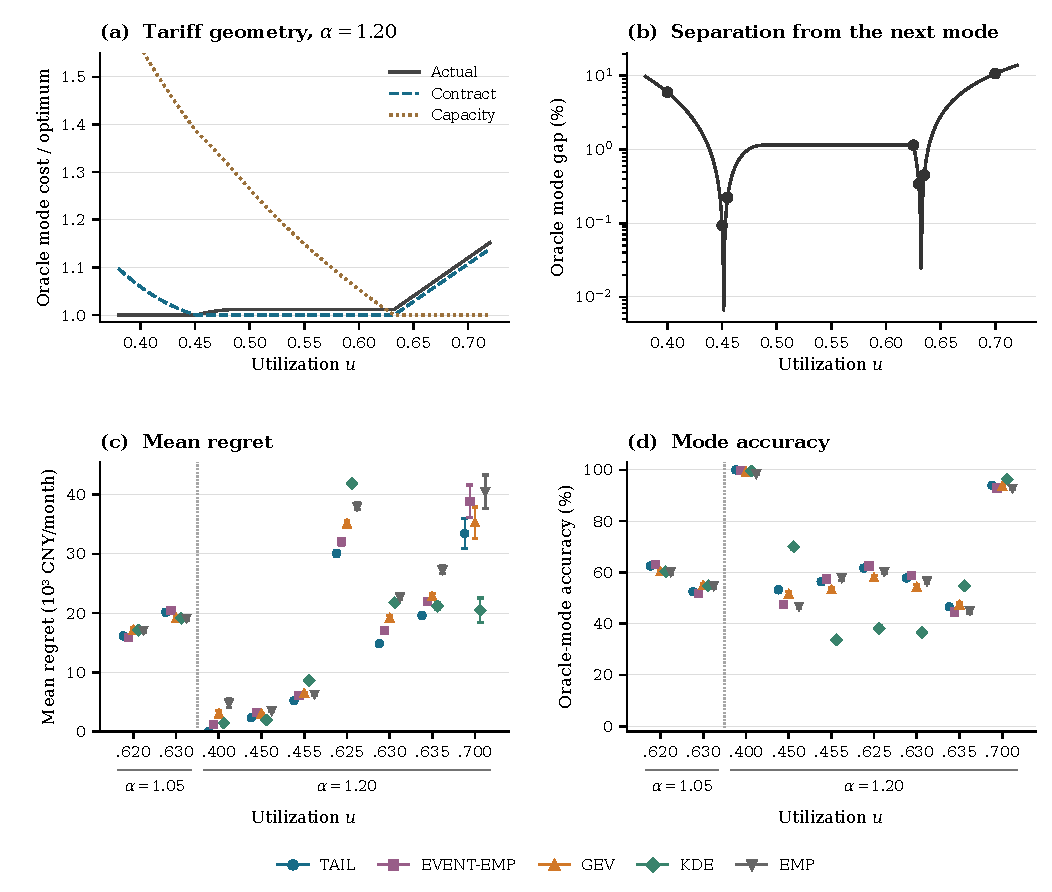
\includegraphics[width=\linewidth,height=0.65\textheight,keepaspectratio]{figures/Figure_1.pdf}
\caption{\textbf{Analytic tariff geometry and primary decision performance.}
\textbf{(a)} Oracle optimized mode costs divided by the best oracle
value and \textbf{(b)} the relative gap between the two lowest oracle
mode values, at $\alpha=1.20$; dots in (b) identify the seven primary
cells at this $\alpha$. The seven displayed cells form the $\alpha=1.20$ subset of the
nine-cell primary tariff design summarized in Table~S13.
\textbf{(c)} Mean full-action regret and pointwise $t$ 95\% intervals
and \textbf{(d)} oracle-mode accuracy with Wilson 95\% intervals for
five methods at nine prespecified cells. Each method--cell summary uses
10,000 independent 24-month histories; fitted laws and histories are
shared across cells. TAIL and EVENT-EMP use event histories; GEV, KDE
and EMP use monthly maxima. The lower panels use equally spaced cell
positions, labelled by utilization and grouped by $\alpha$, rather than
a continuous utilization axis.}
\label{fig:tariff-geometry}
\end{figure}

\subsection{Economic rankings vary with tariff geometry}
\label{sec:results-economic-value}

Statistical fidelity did not produce a single economic ordering.
Under the controlled data-generating process, TAIL had the smallest
median absolute relative $q_{0.99}$ error, $10.09\%$, compared with
$14.30\%$ for KDE
(Table~\ref{tab:table_2}; Figure~\ref{fig:statistical-regret}(a)).
The median stop-loss errors, evaluated at the cell-specific oracle
contract thresholds and averaged over the nine cells within history,
were $28.49\%$ for TAIL, $31.00\%$ for GEV, and $33.55\%$ for KDE.
The association analysis showed a corresponding functional pattern.
For TAIL, Spearman correlations of regret with absolute relative mean,
stop-loss, and $q_{0.99}$ errors were $0.753$, $0.683$, and $0.534$.
The mean-minus-$q_{0.99}$ and stop-loss-minus-$q_{0.99}$ correlation
differences were $0.220$ and $0.149$, with simultaneous familywise
95\% intervals of $[0.203,0.237]$ and $[0.139,0.160]$.
All ten simultaneous intervals comparing mean or stop-loss error with
$q_{0.99}$ error were positive across the five predictive methods
(Table~S7).

Within the monthly-maxima information set, GEV and KDE reversed their
economic ordering across oracle regions. The GEV-minus-KDE mean-regret
contrast was $+0.822$ thousand CNY/month in the actual-demand region
(95\% interval $[0.677,0.967]$), $-3.887$ in the contract-demand
region ($[-4.143,-3.632]$), and $+5.470$ in the capacity region
($[4.874,6.067]$). Within the event-level information set,
TAIL-minus-EVENT-EMP contrasts were $-0.606$, $-1.680$, and
$-2.671$ thousand CNY/month in the same three regions, with all three
95\% intervals excluding zero. Complete regional pairwise contrasts
are reported in Table~S12.

The complete-procedure TAIL--KDE comparison, which also differs in
information resolution, showed the same dependence on tariff geometry.
Its regional mean contrasts were $-0.659$, $-7.379$, and $+4.129$
thousand CNY/month in the actual-demand, contract-demand, and capacity
regions. The capacity-region average combined markedly different
cell-level effects: $+1.004$, $-1.561$, and $+12.945$ thousand
CNY/month at $(\alpha,u)=(1.05,0.630)$, $(1.20,0.635)$, and
$(1.20,0.700)$. At the last cell, TAIL and KDE selected a non-oracle
mode in 600 and 373 of the $10{,}000$ histories. Because the oracle
action there is the singleton capacity mode, every mode-selection error
incurs a discrete mode loss; selections of contract demand can
additionally retain within-contract loss. Table~\ref{tab:table_3}
reports the corresponding method-specific regional regret and
oracle-mode accuracy.

The geometry dependence remained visible beyond the nine-cell primary
design. Figure~\ref{fig:statistical-regret}(e--h) evaluates four
values of $\alpha$ and 19 utilization levels per value, giving
76 tariff cells and 380,000 method--history--cell evaluations.
Both the TAIL--KDE and GEV--KDE cellwise mean-regret contrasts varied
with utilization and oracle mode. Oracle contract demand occurred in
nine crossed-grid cells, all at $\alpha=1.20$; the remaining cells
were assigned to actual demand or capacity. These profiles are
descriptive at the cell level, with history retained as the sampling
unit for inferential comparisons. Complete five-method normalized-regret
and oracle-mode-accuracy profiles are reported in Figure~S8.

\begin{figure}[!htbp]
\centering
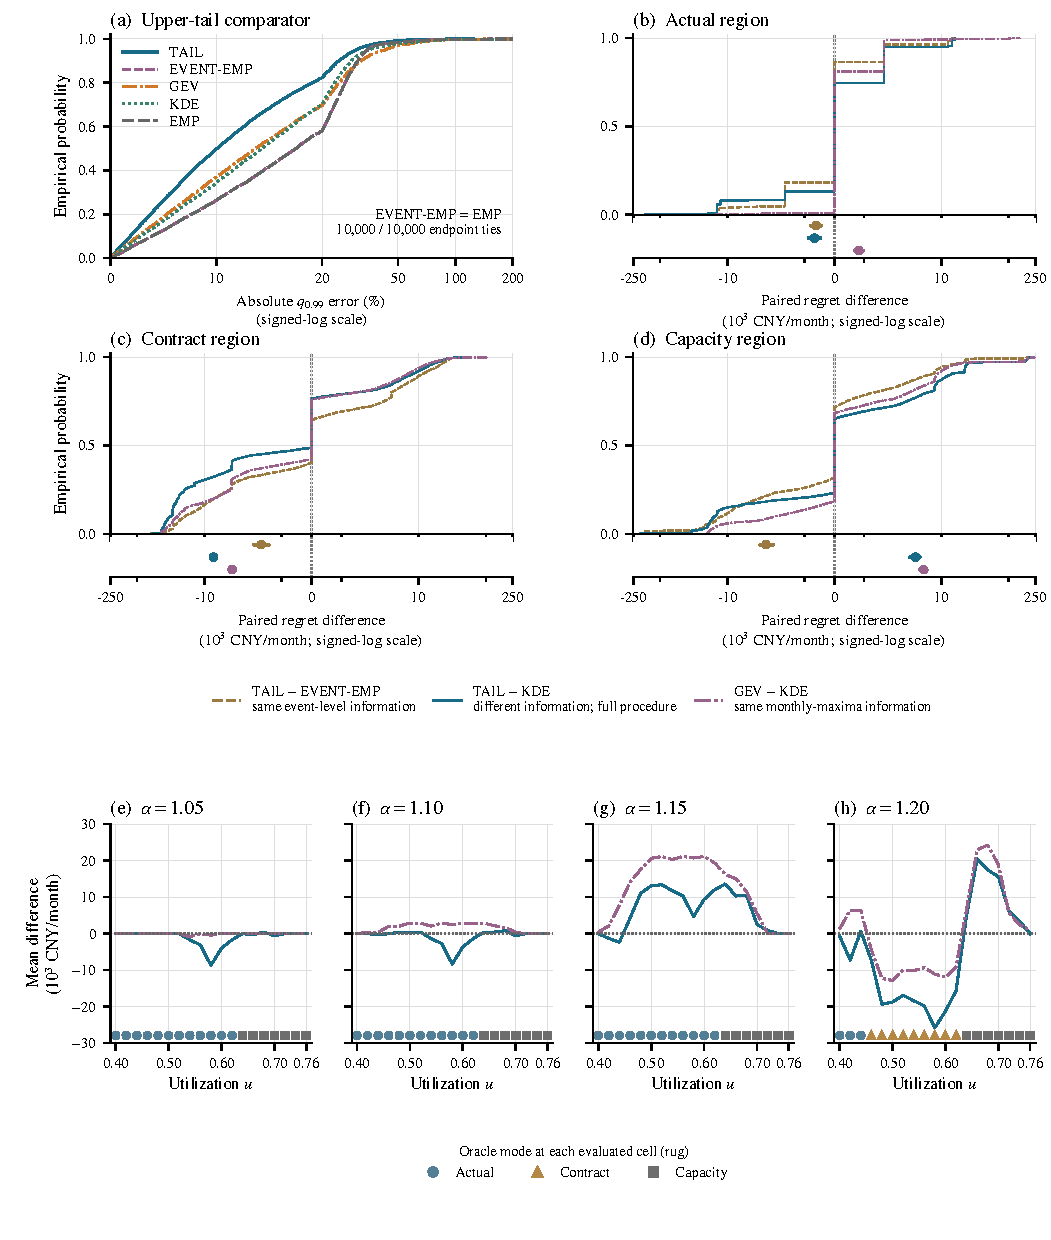
\includegraphics[width=\linewidth,height=0.65\textheight,keepaspectratio]{figures/Figure_2.pdf}
\caption{\textbf{Statistical fidelity and geometry-dependent regret.}
\textbf{(a)} Empirical CDFs of absolute relative $q_{0.99}$ error
over 10,000 histories per method; EVENT-EMP and EMP coincide. The
scale is linear to $20\%$ and logarithmic above.
\textbf{(b)--(d)} Paired full-action regret differences for the
actual-demand, contract-demand, and capacity regions, respectively,
after averaging the three cells within each of 10,000 histories.
Contrasts are TAIL--EVENT-EMP, TAIL--KDE, and GEV--KDE; negative
values favour the first method. ECDFs summarize the paired
differences, with mean contrasts and paired Student $t$ 95\%
intervals ($df=9{,}999$) shown as formal inferential summaries.
Axes are linear within $\pm2$ thousand CNY/month and logarithmic
outside.
\textbf{(e)--(h)} Descriptive mean-regret contrasts over the 76-cell
crossed grid ($\alpha=1.05,1.10,1.15,1.20$; 19 utilization levels
and 1,000 histories per method--cell). Solid and dash-dotted lines
denote TAIL--KDE and GEV--KDE; rugs show oracle modes. Complete
five-method crossed-grid profiles are in Figure~S8, and primary
regional paired contrasts are reported in Table~S12.}
\label{fig:statistical-regret}
\end{figure}

\subsection{Tariff contrasts sharpen demand-scale stability}
\label{sec:results-stability}

The competitor-specific mode-value condition held for $19.52\%$ of
the 450,000 primary decisions, compared with $10.208\%$ for the
scalar $d_{MV}<1$ condition
(Figure~\ref{fig:mode-stability}(a,b)). Neither set contained an
observed tariff-mode error. The difference reflects the information
retained by the two conditions: the competitor-specific condition keeps
each oracle gap and optimized mode-value error separate, whereas
$d_{MV}$ reduces them to a single conservative ratio.

The demand-scale analysis shows a parallel hierarchy. The
contrast-aware radius was never smaller than the mode-wise pairwise
radius and was strictly larger in four of the nine primary tariff cells
(Table~S13). At $(\alpha,u)=(1.20,0.400)$,
$(1.20,0.450)$, and $(1.20,0.455)$ it was three times larger;
at $(1.20,0.625)$ it was 1.5 times larger because the binding
competitor changed from actual demand to capacity. Using the same
numerical $W_1$ upper quantities and solver allowance, the
contrast-Wasserstein check held for $57{,}501$ decisions
($12.778\%$), compared with $26{,}393$ ($5.865\%$) for the
mode-wise pairwise-Wasserstein check and $5{,}329$ ($1.184\%$)
for the uniform-Wasserstein check. No observed mode-selection
violation occurred among rows satisfying any of these numerical
conditions (Table~S14). The numerical $W_1$ quantities and solver
allowances are floating-point constructions rather than
directed-rounding interval bounds.

The exact regret decomposition separates preservation of the tariff
mode from preservation of the complete action. Actual-demand and
capacity modes have no within-mode degree of freedom, so selecting
either oracle-optimal mode gives zero within-mode excess. Contract
demand retains the continuous choice of contract level.
Figure~\ref{fig:mode-stability}(c,d) therefore restricts residual
loss to decisions for which contract demand is both oracle optimal and
selected. Positive within-contract regret can remain even when the
tariff mode is preserved.

\begin{figure}[!htbp]
\centering
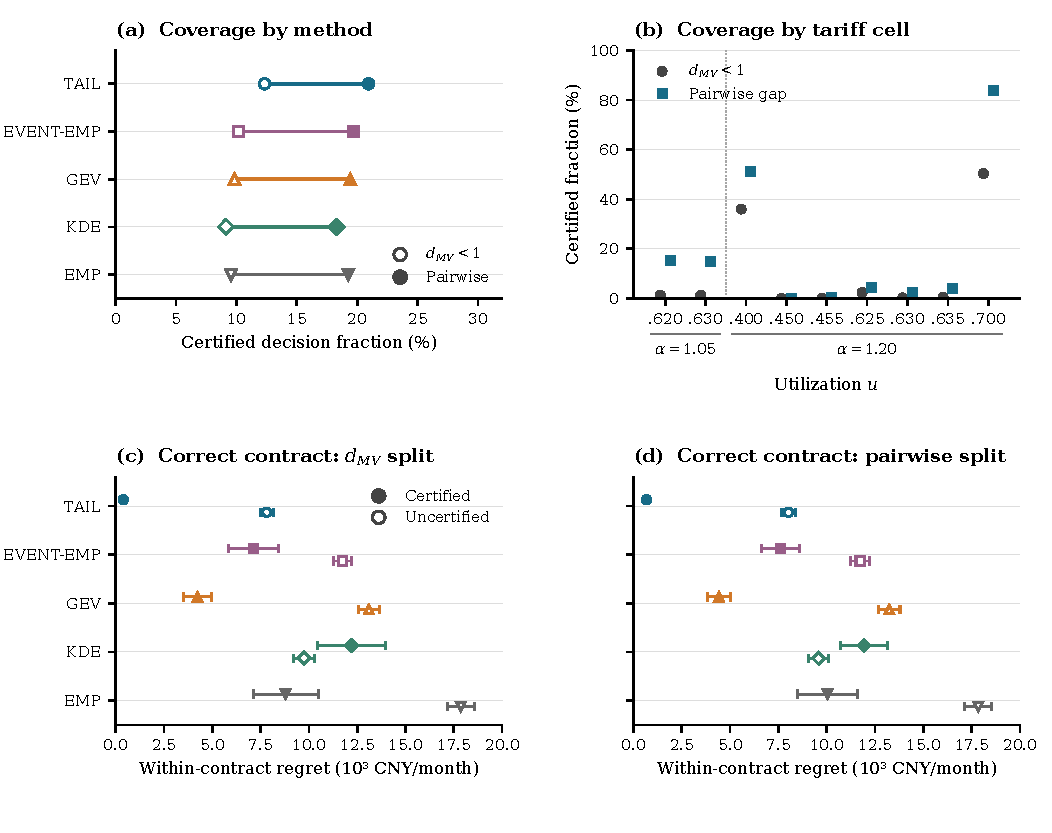
\includegraphics[width=\linewidth,height=0.65\textheight,keepaspectratio]{figures/Figure_3.pdf}
\caption{\textbf{Mode-value stability and residual within-contract
regret.}
The primary analysis contains 450,000 method--history--cell decisions
from 10,000 histories, five predictive methods, and nine tariff cells.
\textbf{(a)} Decision fractions satisfying the scalar $d_{MV}<1$ and
competitor-specific mode-value sufficient conditions, by predictive
method.
\textbf{(b)} Corresponding fractions across the nine primary tariff
cells.
\textbf{(c)} Method-specific within-contract regret among decisions
for which contract demand is both oracle optimal and selected, split
by the $d_{MV}<1$ condition.
\textbf{(d)} The same correct-contract subset split by the
competitor-specific mode-value condition. Panels (c,d) omit
mode-correct actual-demand and capacity decisions because their
within-mode excess is identically zero. Within-contract regret is shown
in $10^3$ CNY/month.}
\label{fig:mode-stability}
\end{figure}

\subsection{Stress designs reveal mechanism-dependent rankings}
\label{sec:results-stress}

The joint negative-binomial--Weibull challenge preserved the
region-dependent economic comparisons under a different count and
severity mechanism (Figure~S7; Tables~S4--S5). For the
same-information event-level comparison, TAIL-minus-EVENT-EMP
mean-regret contrasts were $-28.97$, $-11.71$, and $+7.55$
thousand CNY/month in the actual-demand, contract-demand, and capacity
regions. For the monthly-maxima comparison, GEV-minus-KDE contrasts
were $+5.06$, $-34.32$, and $+1.98$ thousand CNY/month across
the same regions. All six 95\% intervals excluded zero. The two
information-matched comparisons therefore produced different economic
orderings as the oracle tariff region changed.

The physical-pipeline experiment produced a different ordering under
high-amplitude, high-frequency, and clustered-event mechanisms
(Figure~S6; Table~S3). With 24 months of training, mean regret for
KDE-MC-JOINT was $0.842$, $0.948$, and $1.020$ thousand CNY/month
across the three scenarios, compared with $4.451$, $4.311$, and
$3.782$ for TAIL-JOINT. Tail-oriented construction therefore did not
translate into the lowest downstream regret under these alternative
physical mechanisms.

The high-$p^\ast$ analysis varied the tariff target while retaining
the same baseline histories and fitted laws (Figure~S1; Table~S1).
The GEV-minus-KDE contract-region contrast changed direction between
$p^\ast=0.90$ and $0.95$, and its pointwise 95\% interval included
zero at $p^\ast=0.99$; TAIL-minus-EVENT-EMP remained negative at all
three levels. At $p^\ast=0.99$, two of the four contract-region cells
had interior oracle optima and two had lower-bound optima. The
$q_{0.99}$ target is therefore exact for the interior cells, whereas
region-level full-action regret continues to reflect the complete
tariff decision.

Fitted-support sensitivity was limited over the first $1{,}000$ paired
primary histories. Alternative support specifications changed no more
than $0.20\%$ of TAIL mode decisions or $0.40\%$ of GEV mode decisions
in any cell; the largest absolute cellwise paired mean-regret changes
were $0.062$ and $0.726$ thousand CNY/month
(Figure~S3(d--f); Table~S11). Parameter-recovery,
threshold-fixed bootstrap coverage, and physical-clipping analyses are
reported in Figures~S4--S5 and Table~S10.

\subsection{External rankings vary across predictive and tariff targets}
\label{sec:results-external}

The manufacturing-load data produced different point-estimate
rankings across predictive targets
(Figure~\ref{fig:korean-external}(a--d)). K-BLOCK and K-KDE had
lower mean CRPS than K-GTAIL ($0.025390$ and $0.026363$ versus
$0.031017$). For the upper tail, K-GTAIL had the lowest of these
three mean $\operatorname{qwCRPS}_{0.90}$ values
($0.001204$ versus $0.001290$ for K-KDE and $0.001713$ for
K-BLOCK) and the lowest $q_{0.99}$ pinball loss
($0.003212$ versus $0.003262$ and $0.007283$).

Factory-level uncertainty was large relative to these point-estimate
differences. The K-GTAIL-minus-K-BLOCK CRPS contrast was $0.005627$,
with a paired $t$ 95\% interval of $[-0.009534,0.020789]$ across the
eight factories ($df=7$). All 16 pointwise intervals comparing
K-GTAIL with the four baselines across the four predictive losses
included zero (Table~S9). The external predictive results therefore
show target-dependent point rankings together with substantial
between-factory uncertainty.

Figure~\ref{fig:korean-external}(e,f) maps the same forecasts to
hypothetical tariff actions. The panels report normalized next-month
charge contrasts for K-GTAIL versus K-BLOCK and K-GEV versus K-KDE
across the nine tariff cells, using the observed next-month maximum to
evaluate the selected action. The contrasts vary across tariff cells
and their factory-level intervals are wide relative to the cellwise
means, providing a decision-linked complement to the predictive-score
comparison.

Fit-status summaries in Table~S8 show that the prespecified fallback
branches remained active in the rolling procedures. The external scores
and charge contrasts therefore represent the complete predictive
procedures, rather than only origins at which the primary tail fits
were available.

\begin{figure}[!htbp]
\centering
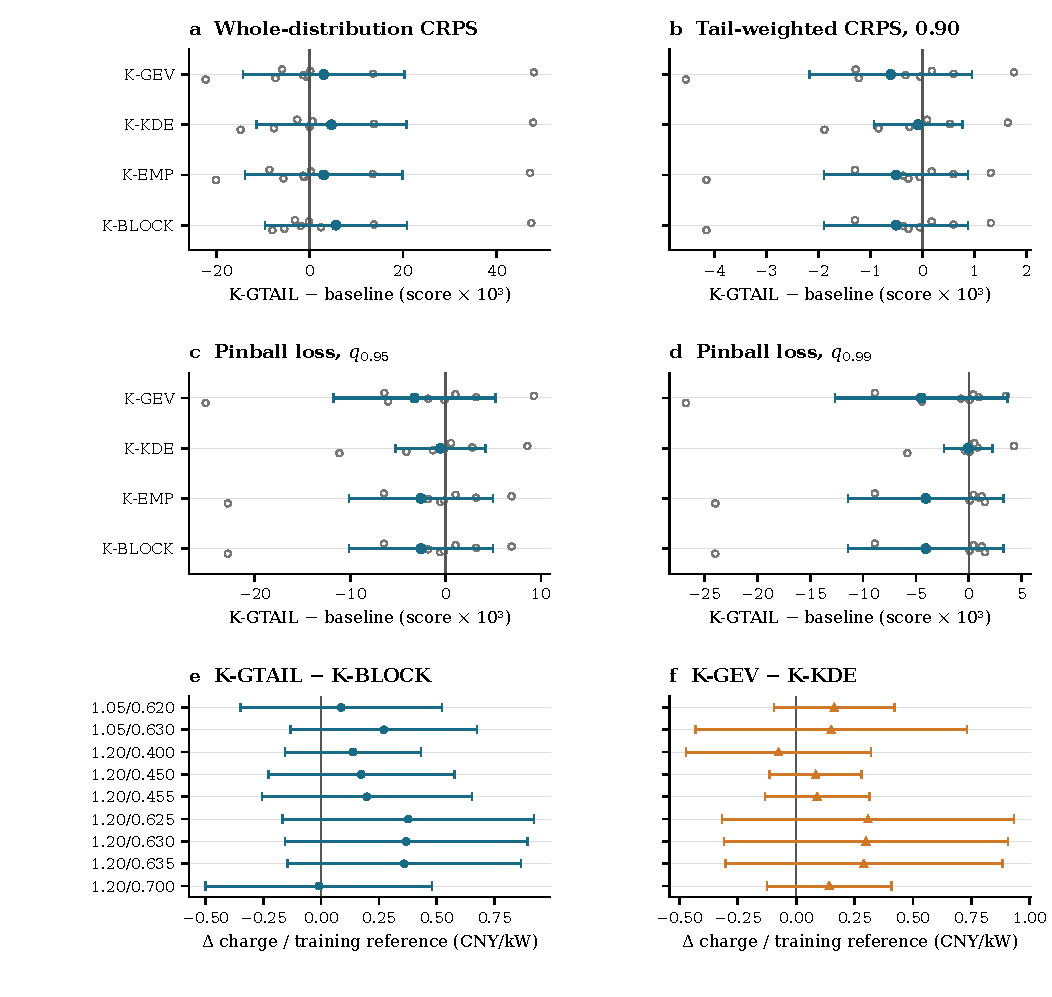
\includegraphics[width=\linewidth,height=0.65\textheight,keepaspectratio]{figures/Figure_4.pdf}
\caption{\textbf{Factory-level predictive-score and hypothetical-charge
comparisons.}
The external analysis uses eight factories with four rolling origins
per factory.
\textbf{(a--d)} K-GTAIL-minus-baseline differences in CRPS,
0.90-tail-weighted CRPS, and pinball loss at the 0.95 and 0.99
quantiles. Open dots are factory-specific differences after averaging
the four origins; filled dots and bars are the mean and paired
Student $t$ 95\% interval across the eight factories
($df=7$). Lower predictive scores are better.
\textbf{(e,f)} Differences in hypothetical next-month demand charges,
divided by the training reference demand, across the nine prespecified
tariff cells. Each charge is obtained by evaluating the selected action
at the observed next-month maximum. The same within-factory averaging
and paired $t$ construction are used. Negative differences favour the
first named method. Oracle regret is defined for the controlled
experiment; panels (e,f) report charge contrasts evaluated on the
external load records.}
\label{fig:korean-external}
\end{figure}

The K-GEV minimum-sample rule assigned the empirical fallback to the
three-, four-, and five-month training origins for all eight factories,
accounting for all 24 fallback predictions. All eight six-month K-GEV
fits passed. K-GTAIL used its primary fit in 15 factory--origin units,
an exponential-tail fallback in 13, and an empirical fallback in four.
All three fitting branches contributed to the reported rolling-origin
scores.



\FloatBarrier
\section{Discussion}
\label{sec:discussion}

Tariff geometry, rather than a global forecast ranking, organizes the
economic comparisons in the controlled study. Within the shared
monthly-maxima information set, the GEV--KDE contrast favours KDE in
the actual-demand region, GEV in the contract-demand region, and KDE
again in the capacity region. The complete-procedure TAIL--KDE
comparison displays the same region dependence, with substantial
cell-level heterogeneity inside the capacity region. This pattern is
consistent with recent decision-focused and application-driven
forecasting studies in which statistical forecast quality and
downstream economic value need not induce the same ranking
\cite{BeykirchEtAl2024,StratigakosEtAl2025,MaciejowskaEtAl2026,HoubenEtAl2026}.
In the present tariff problem, the mechanism is explicit: tariff
geometry changes both the distributional functional entering expected
cost and the separation between competing optimized mode values.

The contract mode makes this functional dependence particularly clear.
Its tariff coefficients determine the probability level
$p^\ast=1-1/(\kappa\alpha)$ and the feasible threshold interval, so the
optimized contract problem has a constrained Expected-Shortfall
representation. A generalized $p^\ast$-quantile locates an optimal
threshold, while the associated upper-tail average determines the
optimized contract value whenever the quantile-optimal set is feasible.
The primary interior targets correspond to probabilities near $0.524$
and $0.583$, rather than $0.99$, which explains why absolute mean and
stop-loss errors are more closely associated with regret than
$q_{0.99}$ error in the baseline design. The high-$p^\ast$ analysis
moves the tariff target into the upper tail and shows that the same
quantile can have different decision implications when feasibility
constraints change the contract optimum. Forecast value therefore
depends on the functional selected by the decision problem, a principle
also emphasized in recent operational evaluations of probabilistic
forecasts \cite{WangEtAl2023,BeykirchEtAl2024}.

Mode separation determines how much distributional perturbation the
discrete tariff choice can absorb. Bounding the optimized mode values
separately gives a valid Wasserstein condition, but direct comparison
of actual demand with contract demand retains cancellation because both
costs respond to the same predictive-law perturbation. The resulting
contrast-aware radius is no smaller than the mode-wise pairwise radius
and is strictly larger in four of the nine primary cells, by as much as
a factor of three. The corresponding numerical sufficient condition is
satisfied by $12.778\%$ of primary decisions, compared with $5.865\%$
under the separate mode-value construction, with no observed
mode-selection error in either passing set. The exact regret
decomposition adds a different distinction: preserving the tariff mode
does not necessarily preserve the full action, because contract demand
retains a continuous contract-level decision after the mode itself has
been selected.

The stress designs show how these mechanisms interact with the
predictive construction and the data-generating process. Under the
negative-binomial--Weibull challenge, both information-matched
comparisons change economic ordering across oracle regions. Under the
physical-pipeline mechanisms, KDE-MC-JOINT has lower mean regret than
TAIL-JOINT in all three 24-month scenarios. The high-$p^\ast$ and
fitted-support analyses separate tariff-target and support sensitivity
from these distributional changes. The manufacturing-load analysis
adds observed industrial demand: whole-distribution and upper-tail
scores produce different point rankings, while factory-level
uncertainty remains substantial and the hypothetical-charge contrasts
vary across tariff cells. Across these settings, the downstream
objective does not support a single predictive construction uniformly.

The analytic Poisson--GPD design makes the complete propagation from
distributional estimation to tariff action observable against an exact
oracle. The alternative count--severity and physical-pipeline designs
show how the economic comparisons change under different mechanisms.
The external analysis adds rolling forecasts of observed industrial
load and evaluates one-month hypothetical charges under the same tariff
family. Longer records linked to actual contract choices and billing
outcomes would extend the present decision-linked evaluation to
realized industrial costs, while covariate-dependent peak-demand models
would allow production state and other operating conditions to enter
the predictive law directly \cite{YuTang2025}.

\section{Conclusions}
\label{sec:conclusions}

This study develops a tariff-specific account of how distributional
estimation error propagates into industrial electricity decisions.
Contract-demand optimization has a constrained Expected-Shortfall
representation at a tariff-implied probability level, full-action
regret separates mode-selection loss from residual within-contract
loss, and direct tariff contrasts yield competitor-specific
Wasserstein stability margins that retain shared distributional
perturbations.

The paired experiments show that economic model rankings can change
with tariff geometry even when the compared procedures use the same
information source. Alternative count--severity and physical-pipeline
mechanisms also change relative performance, while the
manufacturing-load analysis produces target-dependent predictive
rankings and uncertain hypothetical-charge contrasts across factories.
Taken together, the results support evaluating peak-demand forecasts
through the tariff-specific functionals, competing cost margins, and
actions that determine their economic value.

\section*{Supporting Information}
Figures~S1--S8 present, respectively, the high-$p^\ast$ tariff
stress, functional-error and certificate diagnostics, numerical
distribution-to-decision bounds with fitting-support sensitivity,
parameter recovery, physical-clipping sensitivity, physical-pipeline
stress, the joint negative-binomial--Weibull challenge, and crossed
tariff-grid profiles. Tables~S1--S14 provide the corresponding
high-$p^\ast$ comparisons, certificate-conditioned contract losses,
physical-pipeline results, negative-binomial--Weibull results,
Wasserstein numerical quantities, functional-error contrasts,
external predictive summaries, threshold-fixed bootstrap coverage,
fitting-support sensitivity, primary regional paired contrasts,
analytic demand-scale geometry, and numerical sufficient-condition
audit.

\section*{Data and Code Availability}
The controlled analyses in this study are based on synthetic data generated from the stochastic mechanisms described in Sections~4.1 and~4.3. The South Korean manufacturing-load data used for the external analysis are publicly available from Lee, Baek and Kim \cite{Lee2022KoreanFactories} and the accompanying Figshare release \cite{LeeFigshareV9}.

The simulation and model-fitting code, tariff calculations, external
preprocessing, experiment configurations, random seeds, and result
data are available at
\url{https://github.com/riddlehuang05/extreme-demand-tariff-analysis}.
The repository documents the supplied workflows and dependencies in
\texttt{docs/REPRODUCING.md} and \texttt{docs/RELEASE\_SCOPE.md}.
Its \texttt{data/} directory contains indexed source-data files,
including functional-error analyses and solver comparisons. The
accompanying source manifest, derivation map, and figure/table
manifests document source records and panel mappings for the
supplementary figures and tables; the same source files accompany the
article as a source-data supplement. External source data are obtained
from the cited Figshare release under its access terms.

\section*{Conflict of Interest Statement}
The authors declare no conflicts of interest.


\section*{Funding}
This work was supported by the Undergraduate Innovation Training Program of Yunnan University through the Yunnan provincial key-supported project "Quantification and Control Strategies for Intermittent Industrial Energy Waste Based on Extreme-Value Statistics."

\section*{AI-assisted preparation}
OpenAI Codex was used to assist with code development and checking, analysis implementation, manuscript revision, language editing, and preparation of submission materials. The authors take responsibility for the content and interpretation of the work.

\renewcommand{\bibfont}{\normalfont\fontsize{12}{16}\selectfont}
\bibliographystyle{unsrt}
\bibliography{introduction_references}

\clearpage
\begingroup
\centering
\centering
\captionof{table}{Tariff modes, within-mode decisions, and distributional functionals.}
\label{tab:tariff-functionals}
{\tablebodyfont
\setlength{\tabcolsep}{5pt}
\renewcommand{\arraystretch}{1.18}
\resizebox{\linewidth}{!}{\begin{tabular*}{0.98\textwidth}{@{\extracolsep{\fill}}llll@{}}
\toprule
Tariff mode & Within-mode decision & Expected monthly cost & Distributional functional \\
\midrule
Capacity & None & $r_c S$ & None \\
Actual demand & None & $r_d\mu_F$ & Mean $\mu_F$ \\
Contract demand & $D\in[\delta S,S]$ & $r_d\{D+\kappa H_F(\alpha D)\}$ & Stop-loss $H_F(\alpha D)$ \\
\bottomrule
\end{tabular*}}}
\par\smallskip
{\tablefootnotefont\textit{Notes.} The demand quantities $M$, $D$, and $S$ are defined on a common basis. For contract demand, varying $D$ over $[\delta S,S]$ requires the stop-loss transform over the corresponding feasible threshold set $\{\alpha D:D\in[\delta S,S]\}$. After optimization, the contract-demand objective has the constrained Expected-Shortfall representation in Equation~\eqref{eq:contract-constrained-es}; the stop-loss curve is the primitive functional from which this optimized value is obtained.}
\endgroup

\clearpage
\begingroup
\centering
\captionof{table}{Distributional and tariff-functional fidelity in the primary experiment.}
\label{tab:table_2}
{\tablebodyfont
\setlength{\tabcolsep}{4pt}
\renewcommand{\arraystretch}{1.15}
\begin{tabular*}{\linewidth}{@{\extracolsep{\fill}}lrrrrrr@{}}
\toprule
&\multicolumn{2}{c}{$q_{0.99}$ error (\%)}&\multicolumn{2}{c}{Mean error (\%)}&\multicolumn{2}{c}{Stop-loss error (\%)}\\
\cmidrule(lr){2-3}\cmidrule(lr){4-5}\cmidrule(lr){6-7}
Method & Median & Mean & Median & Mean & Median & Mean\\
\midrule
TAIL & 10.09 & 12.22 & 2.82 & 3.34 & 28.49 & 34.02\\
EVENT-EMP & 17.52 & 18.17 & 2.79 & 3.36 & 30.95 & 37.35\\
GEV & 13.73 & 16.63 & 2.98 & 3.55 & 31.00 & 38.03\\
KDE & 14.30 & 16.17 & 2.98 & 3.56 & 33.55 & 44.95\\
EMP & 17.52 & 18.17 & 2.98 & 3.55 & 31.55 & 38.24\\\bottomrule
\end{tabular*}}
\par\smallskip
{\tablefootnotefont\textit{Notes.}
Entries summarize absolute relative errors over 10,000 independent 24-month histories.
For stop-loss error, the nine cell-specific oracle-threshold errors are first averaged within history; median and mean are then taken across histories. Quantile and mean estimates are shared across cells. TAIL and EVENT-EMP use event histories; GEV, KDE and EMP use monthly maxima. EVENT-EMP and EMP have identical left $q_{0.99}$ estimates, at the observed upper support endpoint.}
\endgroup

\clearpage
\begingroup
\centering
\centering
\captionof{table}{Regional decision loss across tariff modes.}
\label{tab:table_3}
{\small
\resizebox{\linewidth}{!}{\begin{tabular*}{0.98\textwidth}{@{\extracolsep{\fill}}>{\raggedright\arraybackslash}p{80pt}>{\raggedright\arraybackslash}p{65pt}>{\raggedright\arraybackslash}p{85pt}>{\raggedright\arraybackslash}p{85pt}>{\raggedright\arraybackslash}p{70pt}@{}}
\toprule
\textbf{Region} & \textbf{Method} & \textbf{Mean regret (thousand CNY/\allowbreak{}month)} & \textbf{Mean normalized regret (\%)} & \textbf{Oracle-mode accuracy (\%)} \\
\midrule
Actual-demand & TAIL & 6.15 & 0.115 & 71.9\\
Actual-demand & EVENT-EMP & 6.76 & 0.127 & 70.0\\
Actual-demand & GEV & 7.63 & 0.143 & 70.3\\
Actual-demand & KDE & 6.81 & 0.128 & 76.6\\
Actual-demand & EMP & 8.47 & 0.159 & 68.5\\
Contract-demand & TAIL & 16.69 & 0.316 & 58.7\\
Contract-demand & EVENT-EMP & 18.37 & 0.348 & 59.6\\
Contract-demand & GEV & 20.18 & 0.382 & 55.1\\
Contract-demand & KDE & 24.07 & 0.456 & 36.1\\
Contract-demand & EMP & 22.34 & 0.423 & 58.4\\
Capacity & TAIL & 24.38 & 0.485 & 64.4\\
Capacity & EVENT-EMP & 27.05 & 0.539 & 63.1\\
Capacity & GEV & 25.73 & 0.512 & 65.2\\
Capacity & KDE & 20.25 & 0.398 & 68.6\\
Capacity & EMP & 28.96 & 0.577 & 64.3\\\bottomrule
\end{tabular*}}}
\noindent{\tablefootnotefont
\textit{Notes.}
Each oracle region contains three prespecified primary tariff cells.
Within each of the 10,000 histories and each predictive method,
cell-level quantities are first averaged over the three cells in the
region and are then averaged across histories. Mean regret is
full-action regret $R_F(\widehat a)$, reported in $10^3$ CNY/month.
Mean normalized regret is $100R_F(\widehat a)/V_F^\ast$.
Oracle-mode accuracy is the percentage of corresponding cell-level
decisions satisfying $\widehat m=m_F^\ast$. Formal paired regional
mean differences and their paired Student $t$ 95\% intervals are shown
in Figure~\ref{fig:statistical-regret}(b--d) and reported in
Table~S12.\par}
\endgroup
\end{document}
